\chapter{The Eastern Indonesian linguistic area}\label{ch:area}

\section{Introduction} \label{sec:area_intro}
Indonesia is one of the linguistically most diverse countries of the world and hosts about 700 languages spread across a vast archipelago with thousands of islands. Stretching from the large islands of Sumatra and Borneo in the far west, once covered with dense rainforests, along the chains of the Sunda-Banda arc system, up to the western part of mainland New Guinea in the east, the territory of today's Indonesia has provided space for a multitude of ethnic groups to evolve and develop a wealth of distinct cultural and linguistic systems. Archeologists, geneticists, and linguists have all contributed evidence that there were several major waves of human migration spreading over the area. The first humans migrating into the archipelago and beyond set forth as early as about 50,000 BCE in the Late Pleistocene \citep{capelli2001}, at a time when Australia, New Guinea and parts of Indonesia were still connected, and formed the prehistoric continent Sahul. These groups eventually reached New Guinea and continued further eastward to the Solomon Islands and southward into Australia. The descendants of these migrants are associated with the ethnic groups of Aborigines in Australia and the Papuans that live on the island of New Guinea as well as in its vicinity. 

The last wave of migrants arrived much later in the Indonesian area, dating back to a time frame around 4,500 BCE \citep{Bellwood1998;Bellwood2007}. These groups were the ancestors of the Austronesian people. They probably originated from South China, migrated further to the island of Taiwan, and from there on followed along the Philippine Islands down southwards (\citealt{Tryon1995}, \citealt{capelli2001}). In the course of their dispersal into the Malay archipelago, their languages eventually replaced the Pre-Austronesian languages or drove them into the interior parts of the islands. Archaeological evidence suggests that the situation was by no means the same across the Indonesian archipelago. While the western islands of Indonesia had only small Pre-Austronesian populations along the coastlines, which must have entered into a serious competition with the Austronesian seafaring people, the opposite appears to have been true for the island of New Guinea, which already hosted a dense population of Pre-Austronesian agricultural groups at the time of the Austronesian advent (\citealt{Bellwood1998}; see also \citealt{Ross2005}). These different conditions probably had a strong influence on the present situation, where most of the Papuan people are found in the mountainous inner parts of New Guinea, with few remaining settlement areas on and off the island of Halmahera in the northern Moluccas and on the islands of Timor, Alor and Pantar in the southeast. Where Austronesian and Papuan groups live in close vicinity, the former are mainly confined to the coastal areas, while the latter often maintain settlement areas further inland. This distribution is particularly visible in parts of Western Papua, where Austronesian speaking areas are located on the Raja Ampat Islands off the Bird's Head, or live in small communities scattered in and around Cenderawasih Bay.

The Eastern Indonesian region can be defined on geographical, biological, and linguistic grounds, all of which show roughly corresponding demarcation lines. Geographically, the area of today's Indonesia and East Timor may be separated into four parts: the Sundaland continental core in the west, the Australian continent in the southeast, the Pacific and the Philippine oceanic plates to the north, and the vast central collision area that is part of the Sunda-Banda arc system (\citealt{Bellwood2007}, \citealt{Hall2009}). It is the Sunda-Banda arc system that forms large parts of what may be depicted as Eastern Indonesia (together with the western part of the island of New Guinea, which geographically belongs to the Australian continental shelf). Among biologists, the transition area between the shelf formations to the east and west has come to be known as Wallacea. Wallacea forms the central part of the Malesian floristic region and its western border is traditionally defined by Wallace's Line (more recently modified by Huxley's line, \citealt{Bellwood2007}, \citealt{Raes2009}; \citealt{Welzen2011} propose to include Java as well). Wallace's line as well as other biogeographical demarcation lines running through Wallacea designate floristic and faunal boundaries beyond which the ratio of oriental species declines while the number of endemic species sharply increases \citep{Bellwood2007}. Wallace's line separates the island of Bali from its neighbour Lombok to the east and runs northward. Alfred Russel Wallace himself was unsure whether to include or exclude Sulawesi (a question that is also of relevance to the delimitation of linguistic Wallacea, see below) and there are two variants of his line, one running through the strait of Makassar, where it divides Sulawesi in the east from Borneo in the west, and another one running east of Sulawesi \citep{Welzen2011}. Figure \ref{map:wallacea} below illustrates the major demarcation lines. Lydekker's line, running along the edge of the Sahul shelf, is usually considered the eastern border of biogeographical Wallacea.

\begin{figure}
\begin{center}
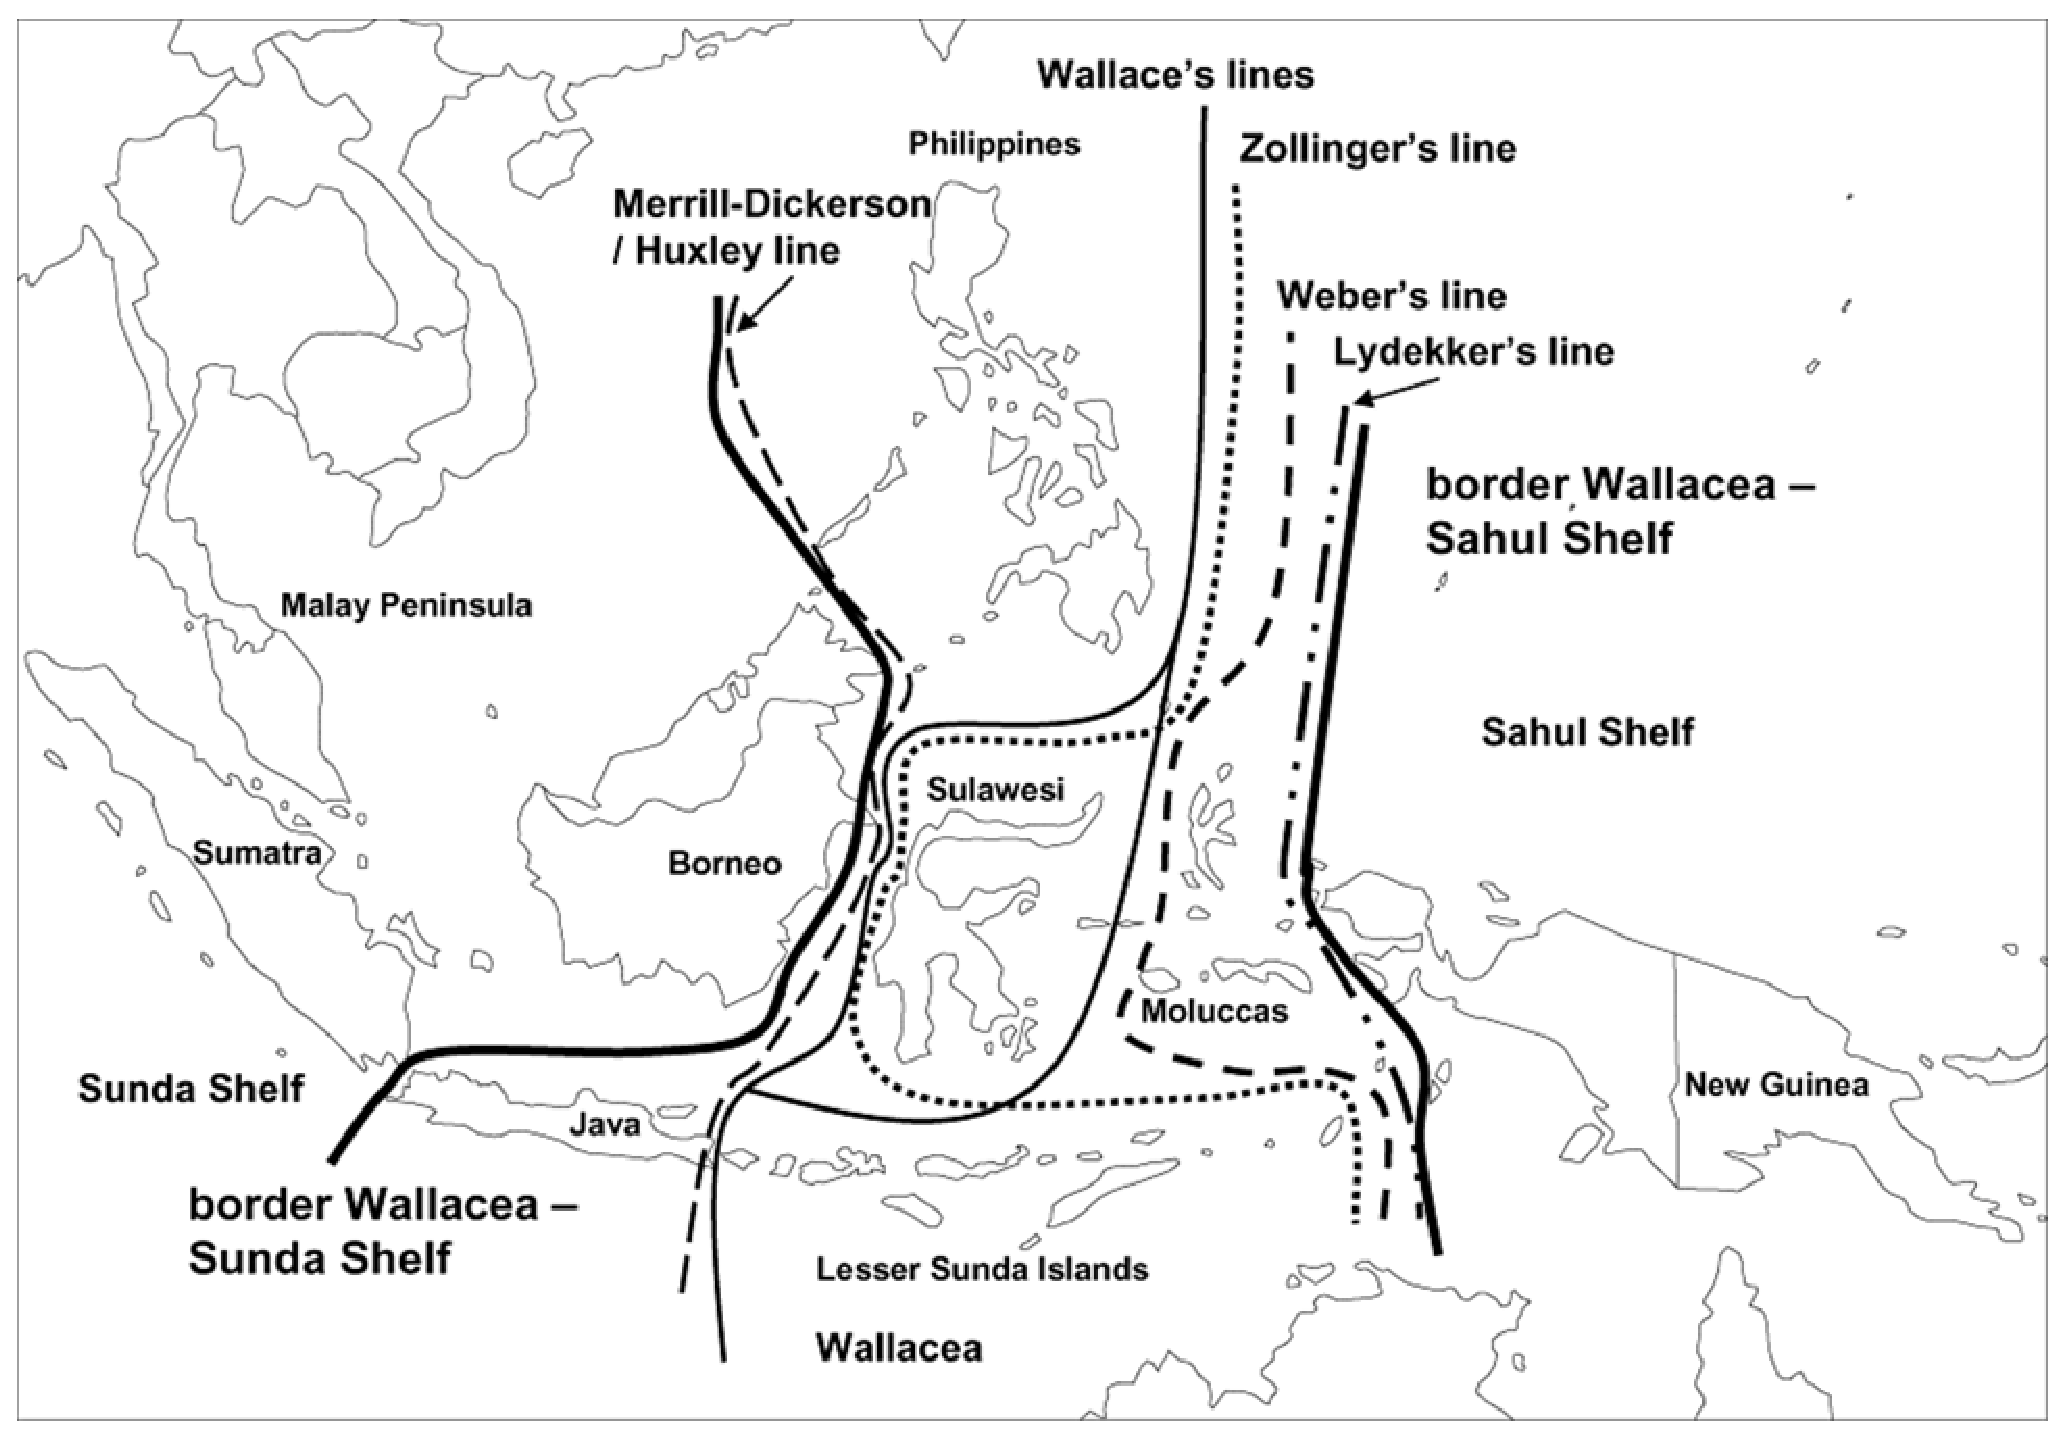
\includegraphics[width=1.0\textwidth]{figures/Wallacea2.eps}
\caption[Biogeographical demarcation lines in insular South-East Asia]{Biogeographical demarcation lines in insular South-East Asia. Wallace's Line is drawn here in two variants, one including Sulawesi, and another one excluding it. Biological Wallacea is traditionally delimited by Wallace's Line in the west, and Lydekker's Line in the east. Reprinted from \citealt{Welzen2011}, Biol J Linn Soc | © 2011 The Linnean Society of London.}\label{map:wallacea}
\end{center}
\end{figure}

Throughout this book, I will consider the western variant of Wallace's line loosely as the western boundary of the Eastern Indonesian area, and mainland New Guinea as the eastern boundary (extending biogeographical Wallacea beyond Lydekker's Line to comprise the Bird's Head area). Moving roughly from west to east, the whole area then consists of Sulawesi, the Lesser Sunda Islands (or Nusa Tenggara) including Timor, the Moluccas, and the western tip of Indonesian Papua. Turning now to linguistic data, we find that the area of Eastern Indonesia as sketched above is supported by both typological and historical-comparative evidence. I will in §\ref{sec:geneticlineage} start with an outline of the diachronic relations, presenting the languages of the EI dataset in the context of their genealogical affiliation as suggested by historical-comparative evidence. In §\ref{sec:typo}, I will then shift the perspective to a typological overview, summarising recent research on Eastern Indonesia as a linguistic Sprachbund. 

\section{Genealogical lineage}\label{sec:geneticlineage}

The languages of Eastern Indonesia share a set of common ancestors, that is, they are in a genealogical relationship. This cannot always be traced by way of the traditional historical-comparative method. It is specifically within the Papuan languages that time depth is a challenging issue: the time frame starting from the point where protolanguages such as Proto Trans New Guinea split up and developed into separate directions up to the contemporary situation in linguistic Papua is tremendous. Given that the advent of Papuan-speaking communities in the New Guinea area dates back about 40,000 years BP, it does not come as a surprise that Papuan linguistics up to today can neither reconstruct a single Proto-Papuan ancestor nor link all branches together. The term `Papuan' is thus to be understood as a cover term for a group of unrelated language families rather than as a genealogical concept. Recent work on the classification of Papuan languages made use of pronoun paradigms as diagnostic evidence for geneaological relations \citep{Ross2005}. Ross identified twenty-three families of Papuan languages all across New Guinea and its vicinity, among them the large Trans-New Guinea (TNG) family.

\subsection{Austronesian languages}

The Austronesian languages constitute a clear monophyletic group, and much work has been done to reconstruct the Proto-Austronesian lexicon, phonology and grammar (recent contributions include, among others, \citealt{Tryon1995}, \citealt{wouk2002history}, \citealt{blust2009austronesian}, see \citealt{adelaar2005austronesian} for an overview). The whole Austronesian language family consists of some 1,200 languages and is considered the largest language family in the world with respect to the number of languages, and the second largest in terms of geographical distribution \citep{adelaar2005austronesian}. Having originated from Taiwan, Austronesian-speaking communities made their way as far west as Madagascar, as far east as Easter Island, and settled much of insular Southeast Asia, Melanesia, Micronesia and Polynesia from Haiwaii in the north to New Zealand in the south. All these groups can be traced back to the primary branch Malayo-Polynesian (MP). The other nine primary branches never ventured out of Taiwan \citep{blust2009austronesian}. MP divides further into Western Malayo-Polynesian (WMP) and Central-Eastern Malayo-Polynesian (CEMP). Both branches comprise some 600 languages. \citet{blust2009austronesian} names as the chief defining feature of WMP the presence of nasal substitution in active verb forms, often leading to segmental changes in the prefix and/or the root (cp. Malay \textit{pukul} `hit' (base form): \textit{me-mukul} (active form); \citealt[30]{blust2009austronesian}). Apart from this characteristic, it is still not clear whether WMP really constitutes a monophyletic group or rather a paraphyletic collection of residual branches that are not CEMP (cf. \citealt[30]{blust2009austronesian}). 

\begin{sidewaysfigure}
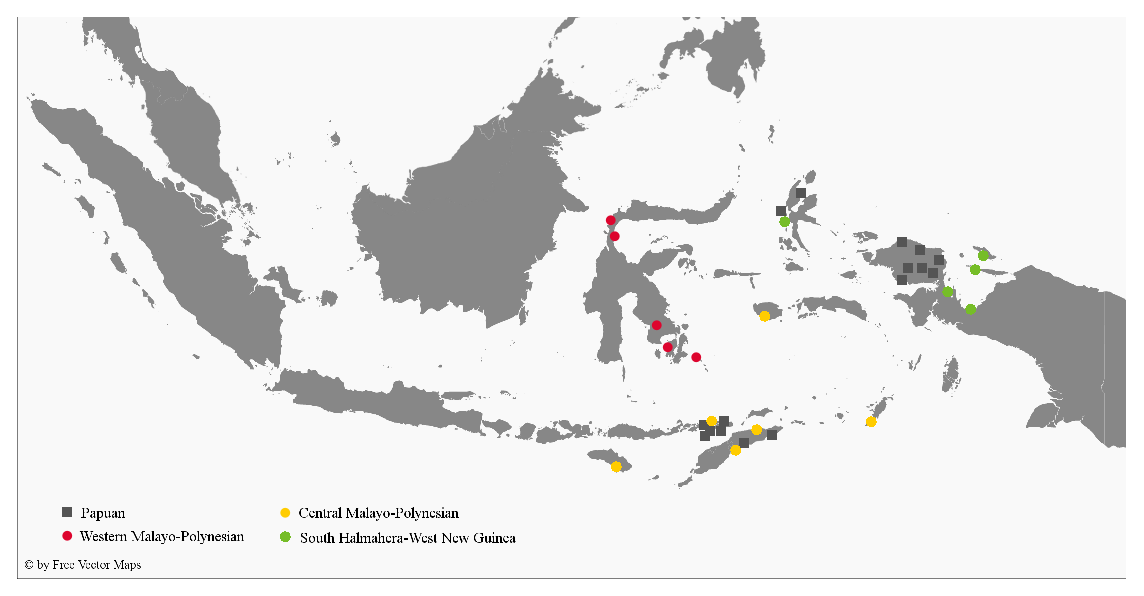
\includegraphics[width=\columnwidth]{figures/Map_overview_klein_Austroaff.eps}
\caption[Geographical distribution of Austronesian languages in the sample]{Geographical distribution of Austronesian languages in the EI sample. Colours indicate genetic affiliation to the different subgroups.}\label{map:Austro}
\end{sidewaysfigure}

CEMP, on the other hand, is firmly supported by phonological, lexical, morphosyntactic and semantic innovations (see \citealt{blust1993central}) and seems now widely accepted. The 600 odd languages divide into an Central-Malayo-Polynesian branch (CMP) with about 120 languages, and an Eastern-Malayo-Polynesian (EMP) branch. The CMP languages are located in the Nusa Tenggara area, comprising the Lesser Sunda Islands from East Sumbawa eastwards, up to the Timor area and beyond into the southern Moluccas, including the Austronesian languages on the western extremities of Bomberai peninsula (Northern Bomberai languages \ili{Sekar}, \ili{Onin} and \ili{Uruangnirin}; \citealt[24]{adelaar2005austronesian}), but not the Halmahera archipelago north of Buru and Seram. Here, as well as in the Bird's Head area and around Cenderawasih Bay, we find 30-40 EMP languages of the South Halmahera-West New Guinea subfamily (SHWNG), which is the sister taxon of the Oceanic languages that have spread eastwards into Melanesia and greater Oceania \citep{blust2009austronesian}. The dividing line between the SHWNG languages in the west and the Oceanic languages in the east runs somewhere through the eastern end of Cenderawasih Bay, leaving \ili{Waropen} in the SHWNG group while the \ili{Sarmi languages} belong to the Oceanic subfamily. Thus all Austronesian languages in EI as defined in this study either belong to WMP, CMP or to SHWNG. Figure \ref{fig:Austro} presents the internal genealogical division of the Malayo-Polynesian languages down to CMP and SHWNG, including the 16 Austronesian languages investigated in this book.

\begin{figure}
\begin{center}
\begin{footnotesize}
\jtree[xunit=8em,yunit=2em]
\! = {Malayo-Polynesian}
:({WMP} {\psframebox{\begin{tabular}{c} \ili{Muna} \\ \ili{Pendau} \\ \ili{Tajio} \\ \ili{Tolaki} \\ \ili{Tukang Besi}  \end{tabular}}}) {CEMP}
:({CMP} {\psframebox{\begin{tabular}{c} \ili{Alorese} \\ \ili{Buru} \\ \ili{Kambera} \\ \ili{Selaru} \\ \ili{Tetun Fehan} \\ \ili{Waima'a}  \end{tabular}}}) {EMP}
:({SHWNG} {\psframebox{\begin{tabular}{c} \ili{Biak} \\ \ili{Dusner} \\ \ili{Mor} \\ \ili{Taba} \\ \ili{Wooi}  \end{tabular}}}) {Oceanic}.
\endjtree
\end{footnotesize}
\end{center}
\caption[The Malayo-Polynesian branch of Austronesian]{Tree diagram of the Malayo-Polynesian branch of the Austronesian language family. Genealogical affiliation after \citealt{adelaar2005austronesian}. Boxed languages belong to the sample of EI languages investigated in this book.}\label{fig:Austro}
\end{figure}
\FloatBarrier

\subsection{Papuan languages}

Quite unlike the Austronesian family, there is up to now no convincing hypothesis that would link the Papuan languages in Eastern Indonesia to a single common ancestor \citep{reesink2005west;klamer2008east}. Papuan languages in EI come in three major areal groupings: (i) the Papuan languages spoken on the islands of Alor and Pantar off the Timorese north coast, as well as the languages located on Timor and the small island of Kisar (\acs{TAP} languages); (ii) the Papuan languages of North Halmahera (NH); and (iii) the Papuan languages of the Bird's Head area, including the isolate \ili{Yawa} on Yapen island in Cenderawasih Bay. Several hypothesis on their genealogical relationship (as well as their connection to the Papuan languages further to the east) have been discussed. The TAP languages have been placed among the Trans New Guinea phylum and links have been postulated between TAP and the West Bomberai languages, most recently by \citealt{Ross2005}, who proposed that they are part of the TNG ``Western Linkage", based on a pronominal innovation in the first person plural \citep[9]{schapper2014intro}. The NH languages, on the other hand, have been placed with the West Papuan languages from the Bird's Head area, most prominently with those of the West Bird's Head family (see \citealt{reesink2005west} for an overview).

\begin{sidewaysfigure}
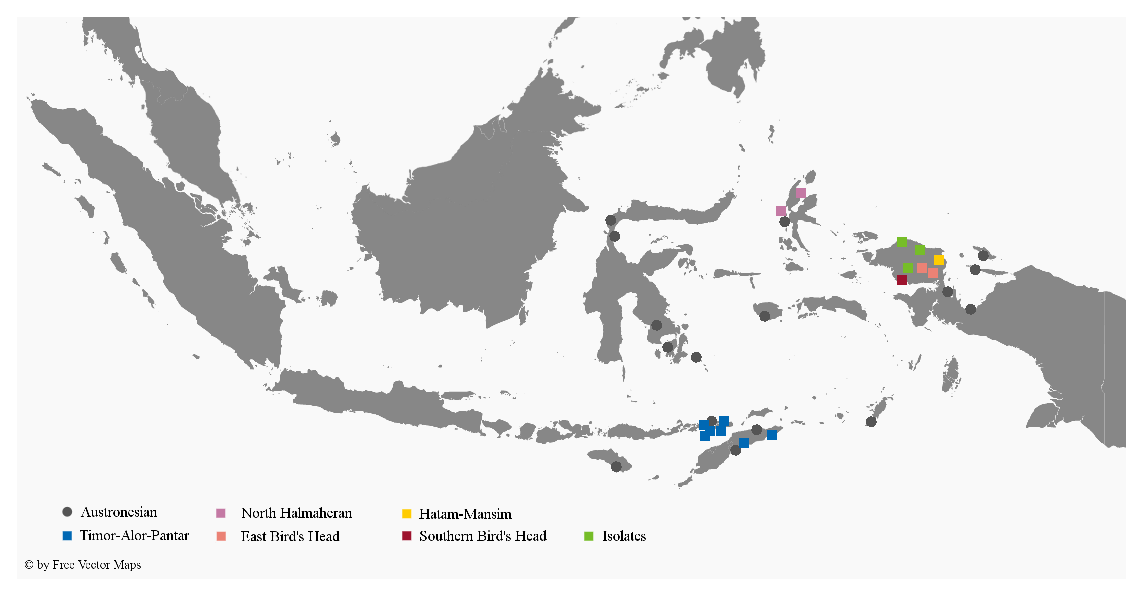
\includegraphics[width=\columnwidth]{figures/Map_overview_klein_Papuaff.eps}
\caption[Geographical distribution of Non-Austronesian languages in the sample]{Geographical distribution of Non-Austronesian languages in the EI sample. Colours indicate genetic affiliation to the different syntaxa. Language isolates are given in green.}\label{map:Austro}
\end{sidewaysfigure}

The TAP languages comprise some 30 languages and divide into two main branches, the Alor-Pantar languages (\acs{AP}) and the Timor-Kisar languages (\acs{TK}). Both subgroups, as well as the TAP branch in general, have recently been established by comparative work \citep{holton2012historical;klamer2014alor}, although a genealogical link between the languages was hypothesized before \citep[7]{schapper2014intro}. While the relationship between the five Timor-Kisar languages seems quite well understood, the interal subgrouping of the AP languages is still under discussion. Figure \ref{fig:timor-alor-pantar} shows a tree diagram for the TAP branch. Seven TAP languages, two TK languages and five AP languages, have been included in the sample.

\begin{figure}
\begin{center}
\begin{footnotesize}
\jtree[xunit=5em,yunit=2em]
\! = {Timor-Alor-Pantar}
:[scaleby=2 1]{Alor-Pantar}!a {Timor}
:{\psframebox{\ili{Bunaq}}} {East Timor}
:{Makasae-Makalero}!b {Fataluku-Oirata}
<left>[scaleby= .5 1]{\ili{Fataluku}} ^<right>[scaleby= .5 1]{\ili{Oirata}}.
\!a = <tri>{AP languages}{\psframebox{\begin{tabular}{c} \ili{Abui} \\ \ili{Kaera} \\ \ili{Klon} \\ \ili{Teiwa} \\ \ili{Western Pantar} \end{tabular}}}.
\!b = <left>[scaleby= .5 1]{\ili{Makasae}} ^<right>[scaleby= .5 1]{\psframebox{\ili{Makalero}}}.
\endjtree
\end{footnotesize}
\end{center}
\caption[The Timor-Alor-Pantar languages]{Tree diagram of the Timor-Alor-Pantar languages, as proposed by \citealt{schapper2014intro}. Boxed languages belong to the sample of EI languages used in this book.}\label{fig:timor-alor-pantar}
\end{figure}
\FloatBarrier

The North Halmaheran language family is supported by lexicostatistic evidence and appears now generally accepted (e.g. \citealt{Voorhoeve1994;reesink2005west}). The languages are located on the northern part of Halmahera, including Morotai and the small volcano islands just off the western shore. NH consists of three related language groups, \ili{Northeast Halmaheran}, \ili{Sahu}, and \ili{Ternate}-\ili{Tidore}, as well as the family level isolate \ili{West Makian} \citep{Voorhoeve1994}. While Voorhoeve listed the Northeast Halmaheran group as a chain of closely related dialects, contemporary research supports the view that the different varieties  form distinct languages rather than dialects. One of the main arguments is that mutual intelligibility is hard to put to the test in areas with extensive multilingualism (see \citealt{holton2003tobelo} on Tobelo; a similar argument is made by Schapper on the TAP languages, see \citealt[3]{schapper2014intro}). Therefore, the rate of real intelligibility would actually be lower if there were no cultural practice of multilingualism. Figure \ref{fig:halmahera} depicts the internal relationship of the NH languages, including the varieties of Northeast Halmaheran. Two languages from this language family have been included in the EI dataset.

\begin{figure}
\begin{center}
\begin{footnotesize}
\jtree[xunit=8em,yunit=2em]
\! = {North Halmaheran}
:{North Halmaheran}!a ({Family level isolate}{West Makian}).
\!a = <left>{Northeast Halmaheran}{\begin{tabular}{c} \ili{Galela} \\ \ili{Loloda} \\ \ili{Modole} \\ \ili{Pagu} \\ \ili{Tabaru} \\ \psframebox{\ili{Tobelo}}  \end{tabular}} ^<vert>{\ili{Sahu}} ^<right>{Ternate-Tidore}{\begin{tabular}{c} \psframebox{\ili{Tidore}}  \end{tabular}}.
\endjtree
\end{footnotesize}
\end{center}
\caption[The North Halmaheran language family]{Tree diagram of the North Halmaheran language family, following \citet{Voorhoeve1994} and \citet{holton2003tobelo}. Boxed languages belong to the sample of EI languages used in this book.}\label{fig:halmahera}
\end{figure}
\FloatBarrier

The third Papuan grouping, the Bird's Head languages of Western Papua, shows a more complicated internal pattern, and the different groups have hitherto resisted the reconstruction of a common ancestor. A fairly traditional approach to the genealogical relationship in the area was the postulation of two main taxa: first, the West Papuan languages, including the Bird's Head languages without the SBH family, and second, the Trans New Guinea phylum, represented in Western Papua by the SBH languages and the West Bomberai subgroup. This dichotomy, however, has recently been called into question as research on the Bird's Head languages has advanced \citep{dol2007grammar}, and more cautious approaches now distinguish a range of smaller sized families \citep{reesink2005west}.

The relationship within some of these subgroups is well established by now. There is evidence that the Papuan languages along the Head's western shore form a coherent group, comprising \ili{Moi}, \ili{Tehit}, \ili{Moraid} and \ili{Seget} (The West Bird's Head family (WBH)). Along the northern shore and further inland, we find a set of unrelated isolates, namely \ili{Abun}, \ili{Mpur}, and \ili{Maybrat}. Finally, there is the East Bird's Head family, consisting of \ili{Meyah}, \ili{Moskona} and \ili{Sougb}, and the \ili{Hatam}-\ili{Mansim} group on the north-eastern part of the Bird's Head. Following \citet{klamer2008east}, we can establish the following list of genealogically related subgroups of which seven languages are part of the EI dataset:


\begin{figure}[ht]
\begin{footnotesize}
\textit{Cenderawasih Bay} \\
(1) \ili{Yawa} (isolate) \\

\textit{Northern Bird’s Head, with three families and three isolates} \\
(2) East Bird’s Head family: \ili{Meyah}; \psframebox{\ili{Moskona}}; \psframebox{\ili{Sougb}} \\
(3) West Bird’s Head family: \ili{Moi}; \ili{Tehit}; \ili{Moraid}; \ili{Seget} \\
(4) \psframebox{\ili{Hatam}} and (extinct) \ili{Mansim} \\
(5) \psframebox{\ili{Mpur}} \\
(6) \psframebox{\ili{Maybrat}} \\
(7) \psframebox{\ili{Abun}} \\

\textit{Southern Bird’s Head} \\
(9) The Trans New Guinea family with two subgroups: \\
– South Bird’s Head, with \psframebox{\ili{Inanwatan}} \\
– West Bomberai: \ili{Iha}, \ili{Baham} \\
\end{footnotesize}
\caption[The Papuan languages of the Bird's Head]{Papuan language families in the Bird's Head area, following \citet{klamer2008east}. Boxed languages belong to the sample of EI languages used in this book.}
\end{figure}
\FloatBarrier

Summing up the genealogical situation in EI, we find both Austronesian and non-Austronesian language communities. While the Austronesian languages are fairly well connected by a shared linguistic history, it has proven difficult to formulate an uncontroversial genealogical reconstruction for the non-Austronesian languages. The TAP languages provide a link to the vast TNG language family in mainland Papua. The North Halmaheran languages as well as the bulk of Papuan languages in the Bird's Head, on the other hand, are not related to TNG. 

The boxed languages from all taxa presented above make up a total of 32 languages, including 16 Austronesian languages and 16 Papuan languages, and together constitute the data source of this study. In the next section, I will put the languages into the context of a shared areal history of mutual contact, resulting in the convergence of features, both Wallacean and Melanesian.

\section{Typological traits}\label{sec:typo}
In most situations where different linguistic communities live in close proximity to one another, there is language contact through trade, inter-marriage, warfare and other kinds of interaction. Such scenarios of contact constitute one of the major forces that cause languages to change over time \citep{thomason2001language}. What is more, such contacts not only lead to language change but over longer periods to language convergence and the formation of linguistic areas in which common structural features diffuse into the different languages. The area that biogeographically forms Wallacea is known for extended periods of language contact between different social groups. \citet[141f.]{schapper2015wallacea} lists archaeological evidence for pre-Austronesian contacts in Wallacea: pelagic fish hook finds from East Timor suggest the existence of a pre-Austronesian seafaring people in the area more than 5,000 years before Austronesian arrival. Rock art motifs from Timor and Bomberai peninsula show similar traits, which suggest prehistoric contact between different communities beginning before 20,000 BP. Obsidian finds from Timor dating back up to 13,000 BP point to ancient inter-island trading routes. Finally, the anthropogenic introduction of Australasian marsupial species into the Wallacea area (for instance the Northern common cuscus \textit{Phalanger orientalis}) confirms human impact across zoogeographical subregions (see also \citealt{Heinsohn2010}).

Moving down to historical times, evidence from trade of natural resources indigenous to the Moluccas, such as clove, nutmeg and mace, suggests that there were ancient trade routes in place as early as 2,000 years ago \citep{klamer2008east}. The 15th century saw the advent of Islam in Ternate and Banda, and in the subsequent centuries, the ``Malayo-Muslim trading network" expanded throughout western Indonesia and well into the eastern parts \citep{klamer2008east}. One of the most important driving forces for inter-cultural contacts in the eastern area was certainly the slave trade and raid routes that were established at the very latest with the rise of the kingdoms of Ternate and Tidore from the 13th century onward \citep{klamer2008east}. These routes extended well into the Bird's Head area where the power and influence of the Sultans was exerted by dominant cultural groups such as the Biak people in the Cenderawasih Bay area \citep[2]{vanheuvel2006} or the Onin ``middle men" along the Bird's Head south coast that had the title \textit{raja} `king' \citep[2]{devries2004}. De Vries reports that these trading networks into the Bird's Head area stimulated situations of extensive language contact:

\begin{quote}There were \textit{raja}'s in the villages Rumbati, Patipi, Ati-Ati and Fatagar and each \textit{raja} had its own section of the Bird's Head south coast where he had some influence through representatives who settled near river mouths. The \textit{raja} of Patipi sent representatives to the Siganoi river mouth where they engaged in slave trade with the Inanwatan people. To get slaves, the Inanwatan raided the interior but also neighbouring coastal peoples like the Yahadian. In exchange for the slaves, they received cloths, iron tools and weapons and guns from the Patipi `middle men'. Although these \textit{raja}'s of Patipi never established a regular government in the Inanwatan area, the Patipi colonists in Inanwatan married local women and Patipi words were borrowed by the Inanwatan language.\end{quote}

The dominant position of these regional agents of the Sultanates had important linguistic consequences all across the region, as their native languages gained the prestige typical for ruling groups. \ili{Biak} and \ili{Onin} thus became local lingua francas in their respective areas of dominance, as did \ili{Ternate} and \ili{Tidore} across the wider Moluccan area, and \ili{Malay} varieties throughout all of Eastern Indonesia. When the first Europeans arrived in the area, they not only found the regional kingdoms to dominate an entire trading economy but also a slave trade along the New Guinean coasts and into the Moluccas and the islands further south that had caused much interethnic mixing. Consequently, many slaves from mainland Papua lived among the populations on Tidore and Ternate. This situation must have led to ``the displacement of Austronesian speakers to non-Austronesian speaking areas, and vice versa" \citep[105f.]{klamer2008east}.

All these historical facts suggest that Wallacea was indeed a place of prolonged and intensive language contact, and, not unexpectedly, this is reflected in shared linguistic features throughout the area. Several authors have discussed sets of common features, and some of them recently suggested a Sprachbund scenario for the area. In the following sections, I will briefly introduce three approaches that highlight the shared linguistic background: Himmelmann's typological profile of Austronesian preposed possessor languages (§\ref{sec:preposed}), Klamer, Reesink and van Staden's approach to East Nusantara as a linguistic area (§\ref{sec:nusantara}), and Schapper's proposal of linguistic Wallacea as a Sprachbund scenario (§\ref{sec:wallacea}). Further Papuan-related features that are found across the Papuan language families in the Bird's Head area and beyond are discussed in \citet{reesink2005west} (briefly reviewed in §\ref{sec:westpapuan}).

\subsection{Preposed possessor languages}\label{sec:preposed}

Working on the Austronesian languages of insular Southeast Asia, \citet{Himmelmann2005austronesian} proposed a typological subdivision of the western Austronesian languages\footnote{The term western Austronesian is a purely geographical expression and should not be confused with the phylogenetic branch of Western Malayo-Polynesian. See \citet{Himmelmann2005austronesian} for further explanation.} (excluding the Oceanic branch) into \emph{symmetrical voice languages} and \emph{preposed possessor languages}. He argues that symmetrical voice and preposed possessors are mutually exclusive in most languages, and that each of these features clusters with other features \citep[113]{Himmelmann2005austronesian}. Symmetrical voice languages are defined by the presence of two or more voice patterns (similar but not equivalent to active vs. passive) none of which can be considered the basic form. The most prototypical representatives of symmetrical voice languages are found within the group of the so-called Philippine-type languages (for instance the well-researched \ili{Tagalog} voice system; \citealt{schachter1976subject}, \citealt{Himmelmann2005tagalog}, \citealt{riesberg2014symmetrical}), which Himmelmann defines as having the following additional characteristics:

\begin{itemize}
\item at least two formally and semantically different \textit{undergoer} voices
\item at least one non-local phrase marking clitic for nominal expressions (e.g. \ili{Tagalog} genitive \textit{ng})
\item pronominal second position clitics
\end{itemize}

These features exclude other symmetrical voice languages like \ili{Malagasy}, \ili{Chamorro} as well as the Tomini-Tolitoli\il{Tomini-Tolitoli languages}, Gorontalo-Mongondic\il{Gorontalo-Mongondic}, Sama-Bajau\il{Sama-Bajau languages}, and \ili{South Mindanao languages} that are spoken in Northern Sulawesi, the southern Philippines and environs \citep[113]{Himmelmann2005austronesian}. The five languages from Sulawesi are the only symmetrical voice languages included in the sample.

Preposed possessor languages, on the other hand, are primarily defined as placing the possessor before the possessum in possessive constructions. This type of language is predominantly found in the eastern parts of Indonesia and appears most often to have either asymmetrical voice alternations or no voice alternations at all. For instance, in the Austronesian language \ili{Waima'a}, spoken in East Timor, the most common possessive construction shows a preposed possessor order, as in \textit{hire buu} (1\textsc{pl}.\textsc{in} ancestor) 'our ancestors' or \textit{mata umo-n} (dead house-\textsc{poss}) `the deceased's house' \citep[31]{bowden2006} \footnote{There is also a less common postposed possessor construction in \ili{Waima'a} where the possessor is overtly marked by final \textit{nini}. This construction, however, is functionally more specific as it appears to focus the possessor, and permits the omission of the possessed entity (see \citealt[32]{bowden2006}}. The dividing line between symmetrical voice languages and preposed possessor languages roughly cuts through the western Lesser Sunda Islands and runs east of Sulawesi, dividing linguistic Eastern Indonesia in two parts: a smaller western portion, consisting of the island of Sulawesi and the westernmost Lesser Sunda Islands Bali, Lombok, Sumbawa and possibly Flores, and a greater eastern part comprising eastern Nusa Tenggara, Timor, the Moluccas and the western tip of mainland Papua. Figure \ref{figure:preposed} shows the distribution of possessive constituent orders in selected languages throughout Indonesia, illustrating the clustering of preposed-possessor languages (blue) in the east and postposed-possessor languages (red) in the west. The map is adapted from the WALS (World Atlas of Language Structure; \citealt{wals-86}) and thus does not display all languages that are part of the EI dataset.

\begin{sidewaysfigure}
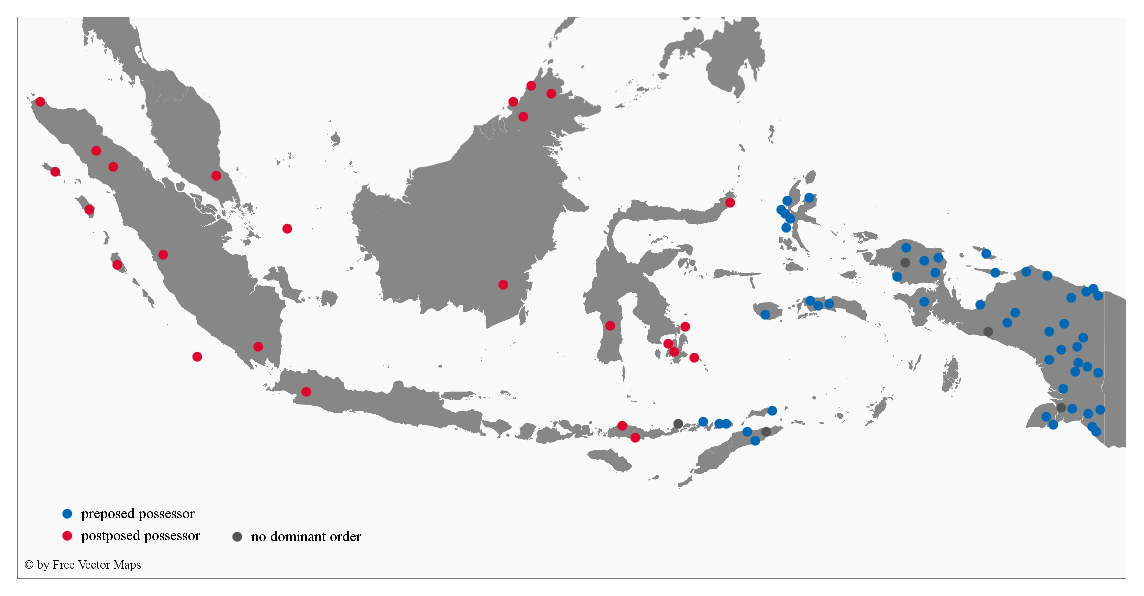
\includegraphics[width=\columnwidth]{figures/Preposed_possessor.eps}
\caption[Order of possessor and possessum in Western Austronesian languages]{Order of possessor and possessum in Western Austronesian languages. Blue circles designate preposed possessor languages, red circle languages show the opposite order with the possessum before the possessor. Grey languages do not have a clear preference. Adapted from \citealt{wals-86}.}\label{figure:preposed}
\end{sidewaysfigure}

What makes the distinction into symmetrical voice languages and preposed possessor languages typologically useful is that these parameters are reported to match with values of further parameters. Table \ref{table:sympre} gives an overview of the feature complex for both typological subgroups. 

\begin{table}[ht]
\begin{center}
\begin{footnotesize}
\begin{tabular}{p{6cm} p{6cm}}
\hline\hline
Symmetrical voice languages & Preposed possessor languages \tabularnewline
\hline
Symmetrical voice alternations & No or asymmetrical voice alternations \tabularnewline
Postposed possessor & Preposed possessor \tabularnewline
No alienable/inalienable distinction & Alienable/inalienable distinction \tabularnewline
Few or no differences between narrative and equational clauses & Clear-cut differences between narrative and equational clauses \tabularnewline
Person marking only sporadically attested & Person marking prefixes or proclitics for S/A arguments \tabularnewline
Numerals/quantifiers precede head & Numerals/quantifiers follow head \tabularnewline
Negators in pre-predicate position & Clause-final negators \tabularnewline
V-initial or SVX & V-second or -final \tabularnewline
\hline
\end{tabular}
\caption[Characteristic features of symmetrical voice and preposed possessor languages]{Characteristic features of symmetrical voice and preposed possessor languages according to \citet[175]{Himmelmann2005austronesian}.}
\label{table:sympre}
\end{footnotesize}
\end{center}
\end{table}
\FloatBarrier

It is certainly not the case that all Austronesian languages in Eastern Indonesia do invariably show all preposed possessor features (person marking, for instance, is absent in a group of isolating Austronesian languages spoken on Timor, see \citealt[175]{Himmelmann2005austronesian}) but chances are high that they have at least some of them. 

\subsection{East Nusantara as a linguistic area}\label{sec:nusantara}

The last section presented evidence that the Austronesian languages in Eastern Indonesia converge on a number of typological features. Turning now to the Papuan languages in the area, we observe that most of these features are shared by them as well, and there have been claims that some of the features listed by Himmelmann are in fact of Papuan origin. \citet{klamer2008east} argue for a linguistic area in Eastern Indonesia which they call East Nusantara (Nusantara is a Malay term meaning `the islands in-between', from \textit{nusa} `island' and \textit{antara} `between'; see \citealt[99]{klamer2008east}). According to their definition, East Nusantara includes all islands along the Sunda-Banda chains, from Flores in the west and Halmahera in the north, up to the Bird's Head region of Indonesian Papua, and is thus roughly consistent with my depiction of Eastern Indonesia above, with one major exception: Sulawesi is excluded from East Nusantara, although the authors note that 

\begin{quote}[t]here is clear evidence that the inhabitants of East Nusantara travelled to places outside the area, and there are genealogical relations between languages of this area and languages outside it. Especially parts of Sulawesi and New Guinea, not included at present, may have to be incorporated later.\end{quote}

In their analysis of East Nusantara linguistic features, the authors argue that the following Papuan features diffused into both Austronesian and non-Austronesian languages (in Eastern Indonesia): alienability, order of possessor and possessum in adnominal possession, and clause-final negators. Evidence that Tone also spread from Papuan to Austronesian languages is considered weak.

The alienability/inalienability distinction, typologically more commonly discussed as part of the more general phenomenon of possessive classification, is absent from western Austronesian languages but occurs in Central-Eastern Malayo Polynesian (CEMP) languages that are spoken in close vicinity to Papuan speaking communitites in Eastern Indonesia \citep[116]{klamer2008east}. The Papuan languages in the area, on the other hand, are reported to have this distinction. Thus, while historical-comparative approaches have attempted to present the alienability distinction as a shared innovation inside the CEMP subgroup \citep{blust1993central}, typologists more recently argued for a Papuan origin. The alienability distinction, and more generally the phenomenon of possessive classification, is a lexically conditioned effect that divides up the noun system of a language into two or more subsets (for instance, in distinguishing between entities with external relation to the possessor vis-à-vis internal relations such as kin, part-whole relations etc). Defined this way, possessive classification can be found as far west as Sulawesi. \ili{Tukang Besi} and \ili{Tajio}, two Sulawesi languages that are part of the sample used for this study, both show different ways of construing (phrasal) possession, and these construals are sensitive to lexical classes. In both languages there is a possessive construction with the possessive determiner \textit{nu}. Consider the following example from Tukang Besi where \textit{nu} connects the possessed item to a possessor.

\ea \label{}
\langinfo{Tukang Besi}{Austronesian}{\citealt[339]{donohue1999}}\\
\gll te kadera nu ama-su\\
\textsc{core} chair \textsc{gen} father-\textsc{1}\textsc{sg}.\textsc{poss}\\
\glt ‘My father's chair’
\z

In Tukang Besi, there are two features of adnominal possession that give rise to an alienable/inalienable interpretation. First, \textit{nu} is preferentially left out when it comes to ``possession of a kin term, or the `possessive relation' expressed between a person and their village, island or ethnic group" \citep[346]{donohue1999}. Second, there is a distinct possessive construction that appears to mark inalienable possession overtly by use of the element \textit{mai}. \textit{Mai} has at least two different meanings or interpretations, depending on the status of the possessed noun. With close kin nouns, the reading is that the item is inalienable from its possessor. The same reading may be invoked with ordinary objects like houses or canoes. The only difference is that in those cases a sense of plurality is associated with the objects. The core system, however, seems to be sensitive to close family kin terms, so that we may say that the set of nouns in Tukang Besi is subdivided into two types (although the \textit{mai} construction is, outside its core semantics with kinship terms, basically a pragmatic device). 

In Tajio, we find a related phenomenon. Here, it is not the possessed noun but the possessor noun class that is differentiated according to lexico-semantic properties. The \textit{nu}-construction marks ordinary inanimate and animate possessors as well as most of the kinship nouns. Four basic kinship terms, however, must be marked with \textit{ni}, and the same is true for pronominal possessed arguments and proper names. Examples (\ref{siama}) and (\ref{tevai}) illustrate the Tajio possessor noun class subdivision.

\ea
\langinfo{Tajio}{Austronesian}{\citealt[227]{mayani2013grammar}}\\
\\
\ea \label{siama}
\glll siama nisari \\
si=ama ni=sari\\
\textsc{hon}=father \textsc{gen}=\textsc{pn}\\
\glt ‘Sari's father’
\ex \label{tevai}
\langinfo{}{}{\citealt[]{}}\\
\gll tevai nujaran \\
te=vai nu=jaran\\
\textsc{nm}=head \textsc{gen}=horse\\
\glt ‘The head of a/the horse’
\z
\z

If possessive classification constitutes an areal feature defining spheres of language contact and the presence of a linguistic area, this area exerts influence beyond the borders of East Nusantara \textit{sensu} \citet{klamer2008east} and into parts of neighbouring Sulawesi. In her discussion of linguistic Wallacea, Schapper notes that ``[t]he Melanesian feature with the widest reach beyond New Guinea is possessive classification" \citep[108]{schapper2015wallacea}, extending far into Melanesia and the Oceanic languages. This eastern spread appears to be weakly mirrored by the possessive classification systems found in Sulawesi languages, beyond East Nusantara proper. Almost all Papuan languages of Eastern Indonesia show the alienability/inalienability distinction. This has led \citet[120]{klamer2008east} to the conclusion that

\begin{quote}[a]lthough it is not a universal feature in the Papuan languages,
the distinction between alienable and inalienable possession is found in a number of different Papuan families [...] and can be seen as a `Papuan trait’.\end{quote}

With regard to the Austronesian languages in the area, Klamer et al. report that the languages east of Timor typically make the alienability/inalienability distinction, while the Timor languages as well as the languages to the west show a more varied pattern. Interestingly, they claim that, among others, \ili{Tukang Besi} does not mark alienability (2008: 120), while Schapper apparently does include \ili{Tukang Besi} in the group of languages that show possessive classification (judging from the map in \citealt[110]{schapper2009bunaq}). As we have seen above, the interplay between \textit{nu} and \textit{mai} at least in some contexts encodes the concept of alienable/inalienable possession, so that Schapper's classification appears justified.

The second feature claimed to be of Papuan origin is the order of possessor and possessum. Klamer et al. show that both Papuan languages with SOV constituent order as well as many SVO Papuan languages have preposed-possessor order, at least with inalienable possession and a full NP possessor \citep[123f.]{klamer2008east}. There are, however, hybrid patterns. In \ili{Maybrat}, spoken in central Bird's Head, the order shifts to possessum-possessor in alienable possession. Consider the following pair of examples. In (\ref{Maybrat_Klamer_b}), the relating element \textit{ro} marks a possessum-possessor construction, while in (\ref{Maybrat_Klamer_a}), inalienable possession shows preposed possessor order without any linking element.

\ea
\langinfo{Maybrat}{Papuan}{\citealt[119]{klamer2008east}}\\
\\
\ea \label{Maybrat_Klamer_a}
\gll fnia m-ao\\
woman \textsc{3}\textsc{u}-foot\\
\glt ‘The woman's foot’
\ex \label{Maybrat_Klamer_b}
\gll amah ro t-atia\\
house \textsc{poss} \textsc{1}\textsc{sg}-father\\
\glt ‘My father's house’
\z
\z

Another feature that seems to be Papuan in origin is clause-final negator placement (post predicate negation in \citealt{klamer2008east}). Recall that this feature is used by \citet{Himmelmann2005austronesian} as a correlate for his preposed possessor languages. Yet from a typological perspective, this should rather co-occur with SOV word order, and is therefore rather unexpected for Austronesian languages with predominant VSO or SVO constituent orders \citep{klamer2008east}. It is, however, well known from several groups of Papuan languages, such as the Trans-New-Guinea languages, the South Bird's Head languages like \ili{Inanwatan}, as well as the Papuan languages of Timor, Alor and Pantar (for instance in \ili{Western Pantar}, \ili{Kaera} and \ili{Sawila}),  languages along the north coast (\ili{Sentani}), some of the Torricelli phylum languages, and East Papuan languages \citep{klamer2008east}. Clause-final negator placement seems also to be present in some of the Papuan languages of Halmahera (\ili{Tobelo} has a predicate-final suffix \textit{-ua}, \citealt{holton2003tobelo}, but see \citealt[131]{klamer2008east}).

In Austronesian languages outside East Nusantara, the typical negation pattern is pre-verbal/pre-predicate or clause-initial. In Eastern Indonesia, however, we do find a number of Austronesian languages with clause-final negation, especially in the eastern parts. \ili{Wooi} is an example, as well as \ili{Dusner}, \ili{Biak} and \ili{Windesi Wamesa} \citep{gasser2014windesi}, all of which show a related formative \textit{va} (which might be a reflex of a borrowed negator from a West Papuan language that has diffused into the area, as \citet{reesink2002eastern} argues). Another example of clause-final negation is the marker \textit{te} in \ili{Taba}, spoken in the Moluccas. These cases notwithstanding, a sizeable amount of Austronesian languages from East Nusantara apparently withstood Papuan influence and still show pre-verbal/pre-predicate negation. Some languages of Timor seem to have retained this pattern (for instance \ili{Waima'a}, see also \citealt[132]{klamer2008east}), and the same goes for some languages further to the west, e.g. \ili{Kambera} (but not \ili{Alorese}), and the Sulawesi languages (for instance \ili{Muna} and \ili{Tukang Besi}). Eastern outliers of the pre-verbal/pre-predicate pattern can also be found in the Moluccas where, for instance, \ili{Selaru} has a pre-verbal negator \textit{lema} \citep[140]{coward2005}. And \ili{Tetun Fehan} (Timor) shows a hybrid pattern involving two general negators \textit{la} and \textit{ha'i}: the former occurs in pre-predicate position, and the latter in post-predicate position \citep[228]{vanklinken1999grammar}.

According to \citet{klamer2008east}, the alienable/inalienable distinction, the preposed possessor order as well as clause-final negation are clearly Papuan traits that have percolated into neighbouring Austronesian languages in the East Nusantara linguistic area. On the other hand, the authors present features that seem to have taken the opposite direction and originated in the Austronesian languages of the area. These are (i) SVO constituent order, and (ii) the inclusive/exlusive distinction. Both features have spread to some of the Papuan languages of the area. All Austronesian languages in the East Nusantara area show SVO word order \citep[113]{klamer2008east}. Among the non-Austronesian languages we find SOV order, a typical Papuan feature, in the Alor-Pantar languages as well as in the Papuan languages of Timor. North Halmahera and the Bird's Head region seem to be more heterogeneous with both SVO and SOV languages present (SVO being more common on the Bird's Head, exceptions are the South Bird's Head languages (SBH), i.e., \ili{Inanwatan}, as well as language isolate \ili{Yawa} on Yapen island). Among the North Halmahera languages (NH), \ili{Sahu}, \ili{Ternate}-\ili{Tidore} and \ili{West Makian} have been reported to have shifted from SOV to SVO, and the same appears to have happened in \ili{Pagu} \citep[114]{klamer2008east}. Closely related \ili{Tobelo}, on the other hand, still shows predominant SOV order, which, as \citet[55]{holton2003tobelo} reports, ``distinguishes Tobelo from most of its NH neighbors". He goes on in noting that VO constituent order is also available in Tobelo, as is the case in most of the Papuan SOV languages.

The inclusive/exclusive oppositon in first person plural pronouns and subject indexers marks a contrast between `we, including you' and `we, excluding you'. Inclusive/exclusive is a widespread feature all across Austronesia, and almost all languages have this contrast \citep{Tryon1995,klamer2008east}. The Austronesian languages in East Nusantara agree with this pattern. Even languages with considerable exposure to Papuan neighbours and clear Papuan traits in their make-up still retain the inclusive/exclusive opposition, for instance Alorese \citep{klamer2011alorese}. Exceptions to the rule are only found in Malay varieties such as the ones spoken in the Northern Moluccas, the Alor-Pantar area \citep{klamer2008east}, as well as in varieties of Papuan Malay on mainland Papua \citep{kluge2014grammar}. With regard to the Papuan languages in the area, \citet[115]{klamer2008east} note that \begin{quote}in East Nusantara, it appears that the inclusive/exclusive distinction for the first person plural, a typically Austronesian feature,
occurs just in those Papuan languages that have had a long history of contact with surrounding Austronesian languages.\end{quote}
This includes the East Bird's Head family (EBH), Meyah and Sougb, as well as the West Bird's Head family (WBH), and the SBH with Inanwatan, but not Maybrat, Abun and Mpur. In the other Papuan taxa of East Nusantara, it is even more widespread: almost all of the Timor-Alor-Pantar languages (TAP) and the Papuan languages of North Halmahera make the distinction with very few exceptions \citep[115]{klamer2008east}. 

\subsection{Linguistic Wallacea}\label{sec:wallacea}

Another approach to defining a linguistic area in Eastern Indonesia has recently been proposed by \citet{schapper2015wallacea}. With biological Wallacea in mind, she argues for a linguistic Wallacea that comprises Nusa Tenggara including Timor, the Moluccas, the
Bird’s Head, and Cenderawasih Bay, but not Sulawesi. Schapper's linguistic Wallacea is thus roughly commensurate with Klamer et al.'s East Nusantara except that Schapper includes the lesser Sunda Islands up to Lombok (conforming to the Wallace line here), while Klamer et al. exclude the islands west of Flores. By taking into account the wider linguistic context east of Wallacea, Schapper argues that some of the features previously discussed as belonging to an Eastern Indonesian linguistic area actually belong to a much larger zone of Melanesian influence. These include negator placement (clause-final negation), noun-numeral (postposed numeral) and genitive-noun (preposed possessor) orders, presence of possessive classification, complex numerals below ten as well as absence of the velar nasal \textipa{N}. The first three features have been mentioned above. Possessive classification includes all types of possessive noun classes and is thus a broader phenomenon than the alienable/inalienable distinction which it includes. Possessive classification is further defined by distinct possessive constructions for each class. It is common in most Austronesian and Papuan languages of Eastern Indonesia and mainland Papua (although many central highland languages and a number of north coast Papuan languages do not have it) and reaches out far into Oceania \citep[109]{schapper2015wallacea}.

The next feature, complex numerals below ten, refers to the compositional nature of numerals between six and ten in many languages that are located close to or on mainland Papua. Complex numerals may either be derived by adding up component numbers (e.g. in \ili{Mambae} (Austronesian, Timor), the term ``eight" is \textit{lim nai telu}
[5+3]), subtracting them (e.g. ``eight" in \ili{Pak} (Austronesian, Admiralty Islands) is \textit{arhuo} [10-2]), or by multiplication (e.g. \textit{\textipa{\*r}ua mbhutu} [2x4] means ``eight" in \ili{Rongga} (Austronesian, Flores); \citealt[113]{schapper2015wallacea}). The distribution of complex numerals stretches from Flores and Sulawesi in the west throughout Eastern Indonesia, continues along the Papuan north coast, up into the Bismarck Archipelago and reaches Vanuatu and New Caledonia in the east \citep[112--4]{schapper2015wallacea}. For Sulawesi, Schapper reports that some South Sulawesi languages show subtractive complex numerals ``eight" and ``nine", while \ili{Makasarese} has additive ``seven" (2015: 113f.). The Sulawesi complex numerals are listed as outliers but may be taken as tentative evidence for a connection between the core area of Eastern Indonesia and Sulawesi.

A final feature of the Melanesian linguistic area is the absence of the phoneme \textipa{N}, a highly frequent phoneme in the vast majority of Austronesian languages, and fairly frequent also in the Papuan languages (roughly one half in Schapper's sample, 2015: 116). The area of absence starts in Timor, Wetar and the islands to the east, moves on to South and Central Maluku, and from there spreads to mainland Papua. The Bird's Head area appears to  predominantly follow the pattern, although \textipa{N} is sometimes found as a nasal allophone. In \ili{Wooi}, word-final nasals turn into \textipa{N}, for instance \textit{ang} 'eat' which retains the alveolar nasal when suffixed with a resumptive object marker (\textit{y-an-i} 'I-eat-it')\footnote{The original nasal is still visible in \ili{Dusner} and \ili{Biak} which have \textit{an} 'eat' (\citealt{ross2008lexicon} give \ili{Proto-Oceanic} *kani and \ili{Proto-Malayo Polynesian} *kaen as reconstructed forms).}.

In order to distinguish the Wallacean linguistic area from the wider 'linguistic Melanesia', Schapper proposes four alternative features that are found across the different language families in the area (and, indeed, even cross the "Papuan-Papuan divide" \citep[124]{schapper2015wallacea}, i.e., occurring in more than one Papuan family in Eastern Indonesia). These features are: (i) semantic alignment of verbal person markers, (ii) neuter gender, (iii) reflexes of \#muku 'banana', and (iv) synchronic metathesis.

Semantic alignment of verbal person markers pertains to systems where arguments are marked differently, depending on their semantic features such as agentivity. Agentivity may result in split-S systems where the sole argument of unergative verbs receives a different encoding from the sole argument of unaccusative verbs, for instance in \ili{Kamang} (Papuan, Timor-Alor-Pantar group, Alor) or in \ili{Taba} (Austronesian, South Halmahera-West New Guinea taxon, Moluccas). Other factors include effectedness, control (volition), aspectual, or others (Schapper 2015: 125). The feature is reported to occur all across linguistic Wallacea, especially in the Alor-Pantar area, on the Aru islands, in Central Maluku and Halmahera, and in some languages around Cenderawasih Bay. \ili{Mori} on the eastern coast of Sulawesi also shows a split-S system \citep{Barsel1994}, differentiating between given subject referents (marked by a pronominal affix on the verb) and new subject referents (marked by a full NP or an independent pronoun). This again hints at a link between linguistic Wallacea and Sulawesi.

Neuter gender systems are defined with regard to a division of the nominal word class along the animacy hierarchy. The label 'neuter' in these systems covers the lower portion of the hierarchy, for instance the nonmale class (e.g. in \ili{Maybrat}), nonhuman (e.g. in \ili{Tobelo}), or inanimate (found for instance in \ili{Ujir}) \citep[128]{schapper2015wallacea}. Neuter gender is predominantly encoded in verbal cross-referencing morphology via prefixes or suffixes. In some Alor-Pantar languages, neuter gender marking also occurs on other parts of speech, for example on demonstratives in \ili{Bunaq}. Yet another form of neuter gender marking appears to be at work in \ili{Wooi} where nonhuman subject referents do not trigger subject agreement on the verb. Consider the following example where subject marking is absent from the main verb \textit{mahoy} (expected \textit{*he-mahoy} `\textsc{3pl}-sit' is not licit).

\ex \label{}
\begingl
\gla payna, hniviay vaw vo, mahoy mahni // \rightcomment{{\small \textbf{Wooi} \textsc{pap}}}
\glb so star \acs{det}:\acs{pl} \acs{foc} sit fit //
\glft `so the stars have the same position
(lit. are seated alike)' \trailingcitation{{\small (HIVIAY\_exp)}}// 
\endgl
\xe

Neuter gender systems constitute a highly marked feature of Wallacea as they are almost completely absent from all other Austronesian and Papuan languages. Exceptions are only found in the \ili{Formosan languages} in Taiwan, as well as in some outliers: \ili{Palauan} (Austronesian, Micronesia) and \ili{Tolaki} (Sulawesi) both show human-nonhuman distinction, and \ili{Kanum} (Papuan, Southern New Guinea) has female-nonfemale gender. \ili{Tolaki} is another case where Sulawesi languages share Wallacean or Melanesian features.

Among the words for `banana', the form \#muku and its variants ``has a striking skewing towards Wallacea" \citep[132]{schapper2015wallacea}.\footnote{I follow Schapper's notation here with the number sign \# marking the form as a generalisation from a set of etyma from partially unrelated languages.} It occurs in some Papuan languages along the western Bird's Head and Bomberai Bay, in Austronesian languages of the Southern Moluccas (with a considerable share on the Aru islands), and finally in the Timor-Alor-Pantar languages as well as in Austronesian languages of the same area as far west as Flores and Sumba. Reflexes of \#muku are, however, completely absent from Halmahera and in the Cenderawasih Bay area.

The last feature, synchronic metathesis, is also a typologically unusual feature that is present in a range of Austronesian languages in the Wallacea area, most of them on Timor, Wetar and adjacent islands to the east. Papuan languages that show synchronic metathesis seem rare and also confined to Timor and the Alor-Pantar area. Synchronic metathesis involves a reversed linear ordering of phonological segments either within a root or as a result of affix-root interaction, for instance the word for 'smile' in \ili{Helong} (Austronesian, West Timor) is realized as \textit{mali} in final position and \textit{mail} in non-final position \citep[134ff.]{schapper2015wallacea}.

\subsection{West Papuan}\label{sec:westpapuan}

\citet{reesink2005west} is concerned with the typological similarities between the different Papuan taxa in Eastern Indonesia (what he calls the West Papuan languages, a geographical term similar to Himmelmann's Western Austronesian) and discusses features that are not only common to the Non-Austronesian languages of the area but also to some of the Austronesian languages. His features may thus also qualify as evidence for a linguistic area. Most of the features he makes use of have been discussed in the previous sections so that I will only mention two further features here: experiential constructions and a specific type of instrument constructions. 

Experiential constructions show peculiar construals in many Papuan and some Austronesian languages in the area. In \ili{Yawa}, the East Bird's Head languages and in some North Halmahera languages, experiencer constructions occur with a 3SG dummy subject and an object experiencer  (of the general form `it hungers me', or `hunger does (strikes) me', \citealt[191]{reesink2005west}). Consider the following example from \ili{Tobelo} where the verb inflects with the objective paradigm, marking the experiencer as the object.

\ex \label{}
\begingl
\gla i-hi-birahi // \rightcomment{{\small \textbf{Tobelo} \textsc{mal}}}
\glb 3-1-happy //
\glft `I am happy' \trailingcitation{{\small (Holton 2003: 39)}}// 
\endgl
\xe

Very similar constructions are also found in the neighbouring languages \ili{Pagu} and \ili{Galela}. In other languages, experiential constructions show nominal construals involving possessive affixes (for instance in \ili{Meyah}, \citealt[192]{reesink2005west}) or body part nouns. To illustrate this feature with Austronesian languages, Wooi construes experiencer constructions involving emotion, affection or cognition (like, love, hate, remember) by using the word for stomach plus a directional or non-directional preposition. Windesi Wamesa does the same \citep[154]{gasser2014windesi}). Here is an example from \ili{Wooi}:

\ex \label{}
\begingl
\gla hane ve ya // \rightcomment{{\small \textbf{Wooi} \textsc{pap}}}
\glb stomach \acs{purp} \acs{1}\acs{sg} //
\glft `He/she remembers me' \trailingcitation{{\small (elicited data)}}// 
\endgl
\xe

Reesink notes that Papuan-style construals of experiential constructions are also present in some Austronesian languages of the Central Moluccas, and in Waropen (Cenderawasih Bay). This seems to indicate that experiential constructions like these may be another feature that helps establish evidence for a linguistic area in Eastern Indonesia, though its geographical distribution most probably does not exceed the Bird's Head area any further than up to the Moluccas in the west.

Another peculiarity in the Bird's Head area is the use of instrument prefixes. These prefixes occur in the East Bird's Head languages and in Hatam, as well as in some of the Austronesian languages spoken around Cenderawasih Bay. Instrument prefixes increase the number of arguments in the clause by one, referring to an argument of the previous clause and marking it as the instrument with which the action is carried out. The restriction is that the argument referred to as instrument is not allowed to be overtly expressed in the same clause. Consider the following examples from Hatam (Papuan) and Biak (Austronesian):

\ex \label{Hatam_ins}
\begingl
\gla di-ba singau di-bi-digo nab // \rightcomment{{\small \textbf{Hatam} \textsc{pap}}}
\glb \acs{1}\acs{sg}-use knife \acs{1}\acs{sg}-\acs{ins}-cut.up pig //
\glft `I use a knife to cut up the pig' \trailingcitation{{\small (Reesink 2005: 194)}}// 
\endgl
\xe
\ex \label{Biak_ins}
\begingl
\gla wai ski-i-ne ko-(vu)k-usr kmam-sko // \rightcomment{{\small \textbf{Biak} \textsc{pap}}}
\glb canoe \acs{3}\acs{trl}-\acs{exs}-this \acs{1}\acs{in}-\acs{ins}-follow father-\acs{3}\acs{trl} //
\glft `The few canoes we use to follow our parents and their relatives' \trailingcitation{{\small (Reesink 2005: 194)}}// 
\endgl
\xe

In all three Papuan languages from the Bird's Head in which such a prefix is attested (Hatam, Meyah, Sougb), it seems to have started as a full verb with the meaning `use/take' or `give' (Reesink 2005: 194). This feature is not present in the other Papuan branches of the area, but it is found for instance in Wooi (which appears to share many Papuan features), as well as in Windesi Wamesa (Gasser 2014: 188ff.). Both languages have the typical multi-clause examples like the ones in (\ref{Hatam_ins}) and (\ref{Biak_ins}), but the mentioned clausal restriction (no overt NP expression of the instrument) is less rigid. It may also appear in pre-predicate topic position within the same clause, as this example from Wamesa shows \footnote{Gasser glosses the prefix \textit{-it-} as applicative and not as instrument as it can also mark a range of aspectual functions. It seems, however, that the term applicative is misleading here as the prefix does not produce verb-argument configuration pairs that are typical for applicative devices in other languages. Only those arguments may be targeted that in the particular context of the utterance may be felicitously interpreted as (non-human) instruments. What is more, in the aspectual uses there is no valency increase whatsoever.}.

\ex \label{}
\begingl
\gla wona=ne-si y-it-awer pimuna=pa-i // \rightcomment{{\small \textbf{Wamesa}}}
\glb dog=\acs{det}-\acs{pl} \acs{1}\acs{sg}-\acs{appl}-hunt pig=\acs{det}-\acs{sg} //
\glft `I use the dogs to hunt the pig' \trailingcitation{{\small (Gasser 2014: 190)}}// 
\endgl
\xe

Summing up the last sections, we have seen that there is ample evidence that the languages in Eastern Indonesia have converged on a number of distinct features from a range of grammatical levels (such as syntagmatic and paradigmatic features, lexical items and even a phonological feature). By mapping the distribution of these features across the area, as shown by Schapper's Wallacean features (2015:  138f.), we can further conclude that the geographical center of the area, the maximal feature density, is found in Timor plus environs on the one hand, and in the Bird's Head area on the other. Some of the features seem more Timorese, for example synchronic metathesis or the distribution of \#muku, while other features like Reesink's experiential constructions and the instrument prefix point to an origin somewhere in the West Papuan influence zone in the Bird's Head. Further research may show that these subareas in fact constitute two different nuclei of linguistic convergence. Further support for these core areas will be presented in chapter \ref{ch:discussion} at the end of this book: One of the main findings is the identification of two `hotspots' of MVC formation in Eastern Indonesia, matching the feature convergence zones in the TAP and the Bird's Head area, respectively. Moving away from these centers, the Moluccas, the lesser Sunda islands west of Alor and Pantar, and even more so Sulawesi, form the western transition zone where Eastern Indonesian features gradually diminish and Western Austronesian features become more and more prevalent. Table \ref{tab:features} below summarizes the features as discussed in the previous sections.

The main purpose of this section was to make the reader aware of the shared linguistic history through which the EI languages have converged on a number of features. Although most of the features fade out as we move away from the central zones of linguistic Wallacea, it seems helpful to also take the more peripheral areas into consideration. As I pointed out at several occasions, it is first and foremost the Sulawesi languages that reflect features of linguistic Wallacea, and should therefore not be excluded at this stage. Just like Wallace himself was unsure about the biogeographical status of Sulawesi, it appears that no consensus has yet been reached as to its linguistic status. As some of the Sulawesi languages quite clearly exhibit MVCs, a selection of five Sulawesi languages has been included in this work. The following section serves to introduce the languages analysed in this book, with a focus on their verbal system as an understanding of this is required to evaluate the findings presented in later chapters.

\FloatBarrier
\begin{table}
\begin{center}
\begin{scriptsize}
\begin{tabular}{l l r r r r r}
\hline\hline
\multicolumn{1}{l}{class} & 
\multicolumn{1}{l}{feature } & 
\multicolumn{1}{l}{Himmelmann} & 
\multicolumn{1}{l}{Klamer et al.} & 
\multicolumn{2}{c}{Schapper} &
\multicolumn{1}{l}{Reesink}\tabularnewline
\multicolumn{1}{l}{} & 
\multicolumn{1}{l}{} & 
\multicolumn{1}{r}{} & 
\multicolumn{1}{r}{} & 
\multicolumn{1}{r}{Melanesian} &
\multicolumn{1}{r}{Wallacean} & 
\multicolumn{1}{r}{}\tabularnewline
\hline
\multirow{4}{*}{\rotatebox[origin=c]{90}{syn}}&negator placement&x&x&x& & \tabularnewline
&noun-numeral&x& &x& & \tabularnewline
&noun-genitive&x&x&x& & \tabularnewline
&word order&x&x& & &x \tabularnewline
\hline
\multirow{8}{*}{\rotatebox[origin=c]{90}{gram}}&(sym) voice&x& & & & \tabularnewline
&inclusive/exclusive& &x& & &x \tabularnewline
&inalienability&x&x& & & \tabularnewline
&possessive classification& & &x& & \tabularnewline
&narrative/equational clause&x& & & & \tabularnewline
&person marking device&x& & & & \tabularnewline
&semantic alignment& & & &x& \tabularnewline
&number-conditioned ablaut& & & & &x \tabularnewline
&experiential constructions& & & & &x \tabularnewline
&instrument prefix& & & & &x \tabularnewline
\hline
\multirow{5}{*}{\rotatebox[origin=c]{90}{lex}}&complex numerals& & &x& & \tabularnewline
&neuter gender& & & &x&(x) \tabularnewline
&\#muku& & & &x& \tabularnewline
&synchronic metathesis& & & &x& \tabularnewline
&pronominal 1SG 2SG& & & & &x \tabularnewline
\hline
\multirow{2}{*}{\rotatebox[origin=c]{90}{phon}}&velar nasal& & &x& & \tabularnewline
& & & & & & \tabularnewline
\hline
\end{tabular}
\end{scriptsize}
\end{center}
\caption[Shared linguistic features in Eastern Indonesia]{Overview of shared linguistic features in Eastern Indonesian languages as discussed by the different authors.}\label{tab:features}
\end{table}
\FloatBarrier

\section{Introduction to the languages}\label{introlang}

The languages of the sample are both strikingly heterogeneous and similar at the same time, depending on which feature is assessed. They are quite different in terms of genetic affiliation as we have seen, but also when it comes to grammatical features. For instance, while some of the Austronesian languages from Sulawesi show (symmetrical) voice systems and employ grammatical formatives on the verb in order to mark off actor and undergoer constructions, voice marking, and voice in general, is largely absent from most parts of Eastern Indonesia and does not figure in the other languages of the sample. At the same time, languages that are not closely related or not related at all, do show strikingly similar features (some of which I have already introduced in section §\ref{sec:typo} on linguistic areas). But there are also other grammatical features that recur across EI: for instance, many Austronesian and Papuan languages make use of person-marking systems on the verb, and they even show similar restrictions on using these person-markers. We find mechanisms at work in Kambera (Austronesian) and in some AP languages (e.g. Abui, Western Pantar, Kaera) where properties of the O argument suppress the use of the argument indexer\footnote{There is a considerable discussion in the literature on the status of person-marking on verbs. Notions like agreement and bound pronouns seem not always applicable from a typological perspective. The term argument indexing (or indexation) has been proposed as a more neutral concept covering both speech-role forms (referencing speech act participants) and allophoric forms (for non-speech role referents) \parencite{haspelmath2013argument}. In what follows, I will adopt this terminology and group the different person-marking systems in EI under the label argument indexing (my use of crossreferencing is interchangeable with indexing).} on the verb. These include, for instance, inanimate, indefinite, or non-specific Os. 

As the focus of this work is on verbs and their function and patterns of combination within the wider clausal and sentential context, the following introduction to the languages will be restricted to properties that will prove to be relevant in the later course of the study. This will give us some idea about what verbs are (like) in the languages of EI. Two properties are of particular importance: the patterns of verbal inflection (collapsed into the notion of headedness in chapter \ref{ch:gram}), and predominant constituent order, as this will be shown to bear on some of the MVC construals found across EI.

\subsection{Sulawesi}

There are five languages from Sulawesi in the sample, covering two distinct areas (see Figure \ref{map:Sul} below). Tajio and Pendau belong to the Tomini-Tolitoli group that is spoken in the province Sulawesi Tengah (Central Sulawesi), stretching along Tomini Bay on the northern peninsula that extends up to Gorontalo and Manado. 

\begin{figure}
\begin{center}
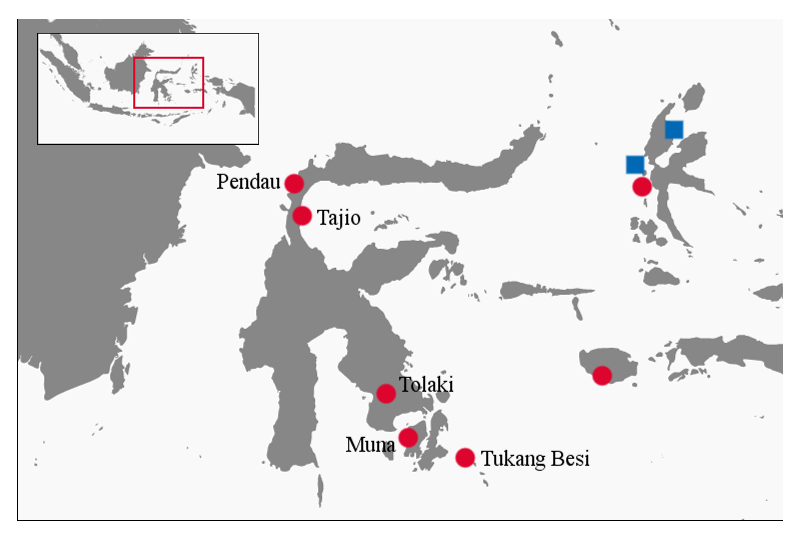
\includegraphics[width=0.7\textwidth]{../Maps/Map_Sulawesi2.eps}
\caption{Distribution of languages from the Sulawesi subarea.}\label{map:Sul}
\end{center}
\end{figure}

Typologically, both languages belong to Himmelmann's symmetrical voice-languages and display a range of Philippine-type features, the most prominent one being a symmetrical voice system with two basic transitive constructions, each of which is marked by overt morphology. Both Pendau and Tajio differentiate between an actor and an undergoer voice construction. In Pendau, the grammatical subject (or pivot\footnote{As the NP sensitive to a given grammatical process is more cautiously called by most research on subjects in Philippine-type systems.}) is defined by position in the preverbal slot, as Quick shows (2007: 124). If the undergoer argument becomes the pivot in an undergoer voice construction, the NP is moved into preverbal position in order to be marked as the pivot. Explicit verbal morphology on the verb specifies the pivot as being the undergoer.

\pex 
\a \label{Pendau_ex1}
\begingl
\gla siama'u nonuju siina'u // \rightcomment{{\small \textbf{Pendau} \textsc{sul}}}
\glb si=ama='u N-pong-tuju si=ina='u //
\glc \acs{nm}=father=\acs{1}\acs{sg}.\acs{gen} \acs{rls}-\acs{sf}-send \acs{nm}=mother=\acs{1}\acs{sg}.\acs{gen} //
\gld \textbf{Pivot=A} {} \textbf{Non-pivot=P} //
\glft `MY FATHER sent my mother.' // 
\endgl
\a \label{Pendau_ex2}
\begingl
\gla siama'u nituju niina'u // 
\glb si=ama='u ni-tuju ni=ina='u //
\glc \acs{nm}=father=\acs{1}\acs{sg}.\acs{gen} \acs{iv}.\acs{rls}-send \acs{nm}.\acs{gen}=mother=\acs{1}\acs{sg}.\acs{gen} //
\gld \textbf{Pivot=B} {} \textbf{Non-pivot=A} //
\glft `My mother sent MY FATHER.' \trailingcitation{{\small (Quick 2007: 124)}}// 
\endgl
\xe

The differenc between (\ref{Pendau_ex1}) and (\ref{Pendau_ex2}) is that the argument \textit{siama'u} in the first example receives an actor interpretation whereas in the second one it is assigned the undergoer role by virtue of the undergoer voice formative on the verb\footnote{Note that Quick argues for this system to be a pragmatic inverse system on a par with inverse systems found, for instance, in some North American languages. Whatever the advantages for such an analysis may be, the Pendau system is in essence one variant of a symmetrical voice system. Both voice constructions are equally basic in terms of morphological marking as well as in terms of frequency (the \textit{ni}-construction was about 20\% more frequent in Quick's analyses, Quick 2007: 580). The term inverse, however, implies that some system is flipped from its normal state to a marked/unnormal one. As this is clearly not what proponents of the symmetrical voice approach want to state about voice systems of this type, I will treat the Pendau system as an `ordinary' symmetrical voice system.}. A further parameter in this construction pair is constituent order alternation. For both the \textit{nong}- and the \textit{ni}-construction there is also a predicate-initial order of constituents available: A \textit{nong}-V O may be replaced by \textit{nong}-V O A, and O \textit{ni}-V A can give way to an alternative order \textit{ni}-V A O (Quick 2007: 366)\footnote{Here and in the remainder of the book, I will use the generalized role labels as introduced by \textcite{Dixon1979} and recently summarized by \textcite{Bickel2011}: S - `sole argument of an intransitive verb', A - `most actor-like argument in a transitive verb', O - `not most actor-like argument in a transitive verb', T - `most patient-like argument in a ditransitive construction' and G - `most goal-like or ground-like argument in a ditransitive construction' (see Bickel 2011: 402ff).}.

Another feature of Pendau (and Tajio) that is shown by the examples above is that the verbs do not carry any person-marking morphology that would cross-reference the arguments with the syntactic functions of the clause. The verb stem does take a lot of formatives at times, basically stem-forming morphology and valency-increasing applicatives and causatives, yet there is no direct link established to the NPs in the clausal context other than by position in the clause (as well as through subtle variation in the assigment of the nominal markers, note for instance the switch from absolute case to genitive case in the actor argument in (\ref{Pendau_ex2})). The Tajio voice system works in a quite similar way, and shows related formatives \textit{noN-/moN-} for actor voice realis/non-realis, and \textit{ni-/nu-} for undergoer voice realis/non-realis (see Mayani 2013 for further details). 

Notably, serial verb constructions are mostly confined to cases where uninflectible directional verbs interact with voice-marked verbs. A first example for illustration is given below in (\ref{tajio01}) from Tajio.

\ex \label{tajio01}
\begingl
\gla sia’u jiopo \textbf{mai} \textbf{nendiis} // \rightcomment{{\small \textbf{Tajio} \textsc{sul}}}
\glb sia’u jio=po mai ne-ndiis //
\glc \acs{1}\acs{sg} \acs{neg}=\acs{cont} go.to \acs{dyn}.\acs{rls}-bath//
\glft ‘I have not gone for a bath yet.’ \trailingcitation{{\small (Mayani 2013: 289)}}// 
\endgl
\xe

Tolaki, Muna, and Tukang Besi form the second group of Sulawesi languages in the sample, and they are all spoken in the far south-east of Sulawesi. While the Tolaki community is located on the tip of mainland south-east Sulawesi, the Muna and Tukang Besi speaking communities live on islands located off the mainland (Muna and Buton are larger islands close to the coast, while the Tukang Besi islands are smaller coral islands forming a chain out into the Banda sea). 

In contrast to Pendau and Tajio, all three south-eastern Sulawesi languages make use of argument indexing systems where pronominal affixes or clitics on the verb crossreference NP arguments in the clause. In Tolaki, both subjects and objects in transitive clauses are crossreferenced by two sets of clitics on the verb. In intransitive clauses, the S argument may receive marking from either class, rendering Tolaki subject crossreferencing a fluid-S system (Mead \& Youngman 2008: 115). Example (\ref{tolaki1}) below shows a transitive clause with a prononimal subject argument and a full NP object that is crossreferenced by the suffix on the verb. Note that certain clause-initial monosyllabic function words may attract the subject clitic, drawing it off the verb.

\ex \label{tolaki1}
\begingl
\gla a-no wohiki-'i ana-ndo // \rightcomment{{\small \textbf{Tolaki} \textsc{sul}}}
\glb and-\acs{3}\acs{sg}.\acs{nom} wash-\acs{3}\acs{sg}.\acs{abs} child-\acs{1}\acs{pl}.\acs{in}.\acs{gen} //
\glft `...and he washed our child'  \trailingcitation{{\small (Mead \& Youngman 2008: 114)}}// 
\endgl
\xe

Tukang Besi has developed a similar system of pronominal subject and object indexing on the verb, yet showing an intricate interplay with case-marking articles of the (pro)nominal arguments in the clause. The basic unmarked transitive construction involves both subject and object indexing on the verb. The O argument follows in postverbal position and is marked with the nominative article \textit{na}, the A argument comes last and is assigned the core article \textit{te} (cp. example (\ref{tukbes1a}) below). If the pronominal object indexer on the verb is left out, however, the case-marking system shows the reverse pattern: now the O argument receives the core case marker \textit{te}, while the A argument is coded as nominative by \textit{na} (as in (\ref{tukbes1b})). Donohue (1999: 53) analysed this system as some kind of Philippine-type voice system, though he pointed out that the 'normal transitive' construction is the one with pronominal object indexing, accounting for about 70\% of the forms found in texts and in fact being the only choice for some verbs. Therefore, the Tukang Besi voice system does not match the characteristics of the symmetrical voice systems found elsewhere in Sulawesi. The following examples illustrate this switch pattern.

\pex 
\a \label{tukbes1a}
\begingl
\gla no-kiki'i-ko (na iko'o) te beka // \rightcomment{{\small \textbf{Tukang Besi} \textsc{sul}}}
\glb \acs{3}.\acs{rls}-bite-\acs{2}\acs{sg}.\acs{obj} \acs{nom} \acs{2}\acs{sg} \acs{core} cat //
\glft `The cat bit you' // 
\endgl
\a \label{tukbes1b}
\begingl
\gla no-kiki'i te iko'o na beka // 
\glb \acs{3}.\acs{rls}-bite \acs{core} \acs{2}\acs{sg} \acs{nom} cat //
\glft `The cat bit you' \trailingcitation{{\small (Donohue 1999: 53)}}// 
\endgl
\xe

The Muna inflectional system is again a bit different. Subject indexing is expressed via three classes of subject prefixes, basically dividing the Muna verbs into three classes: dynamic intransitive verbs mostly take class I prefixes, transitive verbs take class II prefixes, and stative intransitives take class III, albeit with exceptions. Object inflection, on the other hand, is not a crossreference system but involves pronominals attached as suffixes to the verb. Example (\ref{muna1}) illustrates a pair of clauses, where in the first clause an NP object does not trigger object inflection on the verb, while a pronominal object in the second case does. A further interesting feature of class II prefixes is the so-called definiteness shift that occurs with definite objects. If the object is definite, the class II prefix on the verb shifts to a class I prefix (in the example, the shift is from \textit{ne-} to \textit{no-}).

\pex \label{muna1}
\a
\begingl
\gla ne-pepe-mo se-mie // \rightcomment{{\small \textbf{Muna} \textsc{sul}}}
\glb \acs{3}\acs{sg}.\acs{rls}-hit-\acs{prfv} one-person //
\glft `he hit somebody' // 
\endgl
\a
\begingl
\gla no-pepe-kanau-mo // 
\glb \acs{3}\acs{sg}.\acs{rls}-hit-me-\acs{prfv} //
\glft `he hit me' \trailingcitation{{\small (van den Berg 1989: 65)}}// 
\endgl
\xe

Other typical Sulawesi features that occur in all five languages include a bipartite mood marking system on the verb, assigning realis or irrealis mood either through variation of the nasal segment of verbal prefixes, or through changes in the vowel quality of subject agreement prefixes. A further conspicuous feature of most Sulawesi languages is the system of aspectual enclitics attached to the verb. These clitics come in two shapes \textit{=nV/=mV} and \textit{=pV}, the former denoting perfective 'already'-type semantics, the latter one denoting continuative 'still'-type semantics (example (\ref{muna1}) above illustrates the former aspectual in Muna). The placement of these aspectuals poses an interesting challenge to the delimitation of multi-verb sequences as they are sometimes attracted to the first verb, and sometimes to the last one, possibly reflecting underlying constructional differences. Table \ref{table:overviewsulawesi} gives a brief summary of the main verbal features of the five Sulawesi languages.

\begin{table}
\begin{center}
\begin{footnotesize}
\begin{tabular}{l r r r}
\hline\hline
language & constituent order & argument indexing & other verbal inflection \tabularnewline
\hline
Pendau & SV, AVO & -- & voice, mood \tabularnewline
Tajio & SV, AVO/VOA & -- & voice, mood \tabularnewline
\hline
Muna & VS, AVO & S/A crossref & mood \tabularnewline
Tolaki & SV, AVO? & S/A, O crossref & -- \tabularnewline
Tukang Besi & VS, VAO & S/A, O crossref & mood \tabularnewline
\hline
\end{tabular}
\caption[Basic verbal features of the Sulawesi languages]{Overview of basic verbal features of the Sulawesi languages in the data set. Constituent order lists only the basic pattern, pragmatically induced alternative patterns are often also available.}
\label{table:overviewsulawesi}
\end{footnotesize}
\end{center}
\end{table}
\FloatBarrier

\subsection{Nusa Tenggara} \label{sec:nus}

Where the Sulawesi languages in general put most informational load on the verbal head of the clause, for instance by argument indexing formatives, stem-forming morphology, voice and mood markers, the languages of Nusa Tenggara show only limited verbal morphology. Moving from west to east, we can see that while Kambera still retains a rich person marking system on the verb, the Papuan languages of Alor and Pantar only occasionally show verbal person marking, and the Austronesian languages Alorese and \ili{Waima'a} have lost all verbal morphology and have developed towards highly isolating languages.

\begin{figure}
\begin{center}
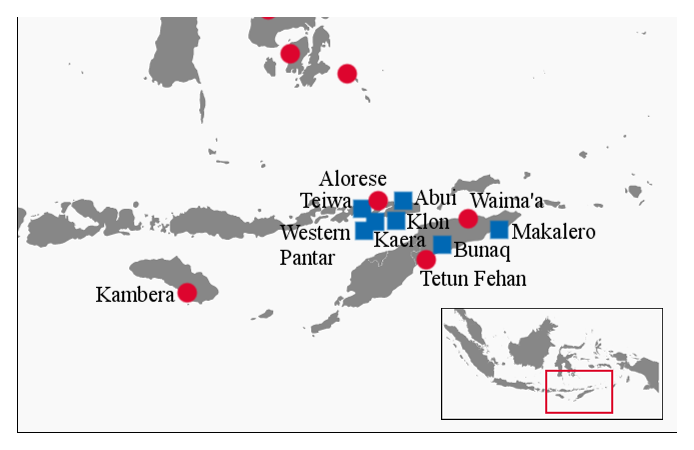
\includegraphics[width=0.7\textwidth]{../Maps/Map_Nusa2.eps}
\caption{Distribution of languages from the Nusa Tenggara subarea.}\label{map:Nus}
\end{center}
\end{figure}  

The Austronesian language Kambera is spoken on the island of Sumba, located about 200km south of the Sunda-Banda island chain. Kambera is the westernmost language of the lesser Sunda islands that has been included in the sample, and accordingly presents some features that are more reminiscent of Western Austronesian languages than of the languages of Eastern Indonesia. The verbal system features four sets of pronominal clitics, each marking one of the `cases' nominative, genitive, accusative, and dative. The crossreferencing system in Kambera is sensitive to certain clitic sequences and to definiteness of the NPs, both of which may influence the clitic choice and combination on the verb. Example (\ref{kamb1a}) shows a canonical transitive construction. Both NP arguments are optional as their properties are coded by clitics on the verb. The two following examples in (\ref{kamb1b}) and (\ref{kamb1c}), however, illustrate two situations which prohibit crossreferencing of all three arguments on the verb. In (\ref{kamb1b}) the sequence of two third person objects causes the expected clitic for the direct object to be omitted. Furthermore in (\ref{kamb1c}), the direct object also fails to be crossreferenced on the verb because it is indefinite.

\pex 
\a \label{kamb1a}
\begingl[glhangstyle=none]
\gla (na tau wútu) na-palu-ka + (nyungga) // \rightcomment{{\small \textbf{Kambera} \textsc{nus}}}
\glb \acs{art} person be.fat \acs{3}\acs{sg}.\acs{nom}-hit-\acs{1}\acs{sg}.\acs{acc} I //
\glft `The big man hit me' // 
\endgl
\a \label{kamb1b}
\begingl
\gla I Ama na-wua-nja$_k$ [na heu na njara]$_j$ //
\glb \acs{art} father \acs{3}\acs{sg}.\acs{nom}-give-\acs{3}\acs{pl}.\acs{dat} \acs{art} one.\acs{clf} \acs{art} horse //
\glft `Father gives them one horse' // 
\endgl
\a \label{kamb1c}
\begingl
\gla (I Ama) na-kei-nja rí // 
\glb \acs{art} father \acs{3}\acs{sg}.\acs{nom}-buy-\acs{3}\acs{pl}.\acs{dat} vegetable //
\glft `Father buys them vegetables' \trailingcitation{{\small (Klamer 1998: 63f.)}}// 
\endgl
\xe

A further conspicuous feature of Kambera is the presence of overtly marked subordinating constructions: a verbal prefix explicitly marks controlled clauses as well as nominalised/relativised subordinate clauses. Overt subordination strategies such as these replace certain types of multi-verb constructions, and set Kambera apart from all other languages in the data set\footnote{A putative further case where a language might be analysed as having non-finite morphology is the \textit{-um-}-infix in Tolaki. However, the occurrence of \textit{-um-} is dependent upon a range of phonological, morphological, syntactic and pragmatic factors, rendering it an unstable indicator for non-finiteness. The data are further complicated by the existence of a homophonous \textit{-um-} morpheme that appears to mark repetitive action in manner of motion verbs. See Mead \& Youngman (2008: 117) for further discussion.}. The following examples illustrate the use of overtly marked subordination in Kambera. Example (\ref{kamb2a}) shows a combination of a nominalised subordinate clause that is linked to the direct object of the matrix clause via the relativiser \textit{pa-}. And in (\ref{kamb2b}) the subordinate clause is marked as a controlled clause by a homophonous \textit{pa-}, indicating that the subject of the matrix clause controls the subject of the embedded clause.

\pex 
\a \label{kamb2a}
\begingl
\gla ta-pakiri-nya$_j$ $[$na pa-tinu-nda$]_{\textsc{np} \textit{j}}$ // \rightcomment{{\small \textbf{Kambera} \textsc{nus}}}
\glb \acs{1}\acs{sg}.\acs{nom}-start-\acs{3}\acs{sg}.\acs{dat} \acs{art} \acs{rel}-weave-\acs{1}\acs{sg}.\acs{dat} //
\glft `We start (with) (it) our weaving' // 
\endgl
\a \label{kamb2b}
\begingl
\gla ta-pakiring $[$pa-tinu-nya na lau haromu$]$ // 
\glb \acs{1}\acs{sg}.\acs{nom}-start \acs{ctr}-weave--\acs{3}\acs{sg}.\acs{dat} \acs{art} sarong tomorrow //
\glft `We start weaving/to weave the sarong tomorrow' \trailingcitation{{\small (Klamer 1998: 338)}}// 
\endgl
\xe

The other Nusa Tenggara languages of the sample are markedly different from the Kambera type. Most of these languages are characterised by two tendencies: first, there is a (massive) reduction in verbal morphology (including person-marking clitics), leading to languages with little or no verbal formatives, and second, if inflection on the verbs is retained we often find irregular inflection patterns. 

If verbal inflection is present, the languages typically exhibit person-marking prefixes or clitics. The Papuan languages show some variation with regard to the number of person-marking paradigms. Schapper (2014) reports that West Alor languages typically have three paradigms, east Alor languages two paradigms and Pantar languages only one paradigm. In terms of verb morphology, we may group the remaining Nusa Tenggara languages in the dataset into two classes. First,  languages that show regular argument indexing in some category or that retain part of their indexing system although the system is not completely obligatory and omission of person-markers is triggered by grammatical or lexical factors: this applies to Abui, Teiwa, Klon, Bunaq, Western Pantar, and Kaera. And second, languages that have either lost their verb morphology completely or still display remnants of person-marking but only under very limited phonological or lexical conditions. This pertains to Makalero, Tetun Fehan, Alorese and \ili{Waima'a}, with the former two showing residual marking patterns and the latter two being (almost) completely isolating. All three Austronesian languages go in this second group. For the Papuan languages of TAP, \textcite{klamer2012development} summarise the number of person-marking paradigms and the alignment system. I show here only the languages that are in the dataset.

\FloatBarrier
\begin{table}
\begin{center}
\begin{footnotesize}
\begin{tabular}{l l l l}
\hline\hline
island & language & no. of prefix paradigms & alignment \tabularnewline
\hline
Pantar & Western Pantar & 1 & split-S \tabularnewline
 & Teiwa & 1 & accusative \tabularnewline
 & Kaera & 3 (1) & accusative \tabularnewline
 Alor & Klon & 3 & split-S \tabularnewline
 & Abui & 5 & split-S \tabularnewline
 Timor & Bunaq & 1 & accusative \tabularnewline
 & Makalero & (1) & (accusative) \tabularnewline
\hline
\end{tabular}
\caption[Overview of TAP prefix paradigms and alignment types]{Overview of TAP prefix paradigms and alignment types (taken from Klamer and Schapper 2012: 178, the Kaera data were added from Klamer 2014a: 128).}
\label{table:TAPprefixalign}
\end{footnotesize}
\end{center}
\end{table}
\FloatBarrier

Abui is the language with the most abundant verb morphology in the TAP group. Abui has both person-marking prefixes and aspectual suffixes on the verb, showing more formative load on the clausal head than is found in most of the other TAP languages. As in other Papuan languages of the area, it is only undergoer arguments that may be crossreferenced by bound pronouns on the verb. A arguments are always expressed by free forms. A feature that seems quite common in the Nusa Tenggara area is that the person-marking systems found on the verbs regularily interact with certain properties of the crossreferenced argument. We have already seen that in Kambera indefinite arguments fail to attract a crossreferencing clitic on the verb. This is mirrored in Abui and other TAP languages by similar interaction mechanisms. In Abui, person-marking is found to be sensitive to contrasts in specificity. For instance, the two object referents in example (\ref{abui1}) evoke different crossreferencing patterns. While the amount of wood is non-specific in the first clause and thus no clitic appears on the verb, it is given a specific reading in the second clause by means of the undergoer clitic\footnote{Class II clitics are referred to as `locatives' by Kratochvíl, and comprise ``prototypical locations, including the
benefactives and malefactives (human location), theme (location of the event), and
purpose (location in time)" (2007: 188). Argument indexing in Abui thus includes a range of non-prototypical core arguments exceeding the number of argument roles that are reported to be indexed in other TAP languages.}.

\pex \label{abui1}
\a
\begingl
\gla maama bataa fak-d-a // \rightcomment{{\small \textbf{Abui} \textsc{nus}}}
\glb father wood break-hold-\acs{dur} //
\glft `father splits wood’ // 
\endgl
\a
\begingl
\gla maama bataa he-fak-d-a // 
\glb father wood \acs{3}II.\acs{loc}-break-hold-\acs{dur} //
\glft `father splits the wood, (the nearer defined quantity of wood)’ \trailingcitation{{\small (Kratochvíl 2007: 179)}}// 
\endgl
\xe

Two further characteristics of the Abui grammar become apparent in the example pair (\ref{abui1}): first, there is a set of aspectual suffixes that attach to the verb. These suffixes are not obligatory in the sense that every verb has to have one. Yet if a verb takes one, there is a constraint concerning the stem allomorph of the verb: Verbs in Abui show stem alternations. These alternations affect the coda and express either completive (final boundary), continuative (no boundary) or inceptive events (initial boundary). That is, aspectual encoding in Abui is at least distributed across two different grammatical layers. Second, Abui not only has a great wealth of SVC constructions on the syntactic level but, according to Kractochvíl's analysis, also has another layer of verb combination, which he names complex verb (formation). Just like \textit{fak} `break' and \textit{d} `hold' are argued to yield \textit{fak-d} `split' in (\ref{abui1}), verb roots are fused and seem to interact in non-trivial ways with the syntactic layer of verb combinations. This complexity in verb formation would be quite exceptional (reminiscent of the Kalam verb system) and is otherwise absent in both AP languages as well as in the other languages of EI.

Turning to the other languages in this group, we find that for instance Western Pantar has a single set of argument indexing prefixes that are obligatory with one (small) set of verbs, optional with another (the majority), and illicit with still other verbs (basically stative intransitives, Holton 2014: 76). Depending on the specific verb, the prefix may either denote an undergoer argument (O or G), or, in some cases, two prefixes occur in sequence with the first one marking the A argument and the second one the O argument, as in (\ref{wp01}). NP arguments may optionally stand in apposition to a person-marking prefix (cp. (\ref{wp02a})) but may also be dropped. The person-marking system is sensitive to animacy contrasts. If the undergoer referent is inanimate, no co-referential pronoun may occur next to the bound prefix on the verb (\ref{wp02b}).

\ex \label{wp01}
\begingl
\gla ke'e pi-ga-ussar // \rightcomment{{\small \textbf{Western Pantar} \textsc{nus}}}
\glb fish \acs{1}\acs{pl}.\acs{in}-\acs{3}\acs{sg}-catch //
\glft `We are catching fish' \trailingcitation{{\small (Holton 2014: 77)}}// 
\endgl
\xe

\pex 
\a \label{wp02a}
\begingl
\gla nang bla ga-niaka // \rightcomment{{\small \textbf{Western Pantar} \textsc{nus}}}
\glb \acs{1}\acs{sg}.\acs{act} house \acs{3}\acs{sg}-see //
\glft `I saw the house' // 
\endgl
\a \label{wp02b}
\begingl
\gla *nang gaing ga-niaka // 
\glb \acs{1}\acs{sg}.\acs{act} \acs{3}\acs{sg}.\acs{ug} \acs{3}\acs{sg}-see //
\glft  \trailingcitation{{\small (Holton 2014: 77)}}// 
\endgl
\xe

Kaera, a neighbour to Western Pantar and Teiwa on Pantar island, has a similar indexing system. Transitive verbs in Kaera fall into three classes which either always take a person-marker to encode O, or optionally take a person-marker, or never express O with a prefix but only with a free NP. This pattern looks quite like the Western Pantar system in that it depends on the verb lexeme whether or not a prefix is required. Interestingly, however, among the smallish class of five verbs in Western Pantar that obligatorily trigger indexing are two verbs, \textit{-niaka} `see' and \textit{-kkang} `hit' (Holton 2014: 77), the equivalents of which in Kaera belong just to the opposite class: \textit{lal-} `see' and \textit{kup-} `hit (thing, person)' refuse bound O-constituents on the verb. 

Another piece of verbal morphology in Kaera occupies the suffix slot: it may be either filled with a marker of clause-final position, or with one of three aspectual suffixes. The phonological shape of the verb root determines whether or not the clause-final marker \textit{-o} is attached or not. Example (\ref{kaera1}) contrasts two clauses. In the first clause, the verb receives the clause-final marker due to its position at the end of the clause. In the second clause, the verb is followed by an aspectual and therefore not marked with \textit{-o}, but instead with one of the aspectual suffixes that are restricted to non-final position verbs.

\pex \label{kaera1}
\a
\begingl
\gla ging tei gu patak-o // \rightcomment{{\small \textbf{Kaera} \textsc{nus}}}
\glb \acs{3}\acs{pl} tree that cut-\acs{fin} //
\glft `They cut that wood' // 
\endgl
\a
\begingl
\gla ging tei gu patak-i sei // 
\glb \acs{3}\acs{pl} tree that cut-\acs{prfv} \acs{comp} //
\glft `They have cut that wood' \trailingcitation{{\small (Klamer 2014: 142)}}// 
\endgl
\xe

Klon, Teiwa and Bunaq basically all show variations of these patterns. Teiwa indexes animate O arguments with prefixes on the verb, and has a reduced reality status inflection pattern consisting of just one morpheme, \textit{-Vn}. It marks ``whether an event has been realized (`realis status') or not (`irrealis status')" (Klamer 2010: 245). The latter is zero marked in Teiwa. As the difference between a zero-marked irrealias and a potential bare verb cannot be ascertained from the published data, this feature causes serious problems in determining whether a given verb in a MVC is in fact meant to be inflected or not. S encoding in intransitive clauses is more straightforward in Teiwa than in other TAP languages: There is no semantic alignment, and the subject of unaccusative clauses is formally marked just the way subjects of unergative clauses are (Klamer 2010: 169). Klon, on the other hand, showing the familiar subcategorisation into obligatory and optional O indexing verbs, does have a semantic alignment system. Some intransitive verbs always take an actor argument, some always take an undergoer argument, and some verbs can either take an actor or an undergoer argument. According to Baird, alignment choice in Klon is effected by the parameters performance, effect, instigation, control and affectedness (2008: 52). Among the group of alternating intransitives, we find for instance that \textit{g-emeq} (\textsc{3ug.I}-not.want) means `she (inherently) doesn't want' while \textit{ga emeq} (\textsc{3sg.act} not.want) translates as `she (decidedly) doesn't want'. Bunaq essentially shows the same argument indexing system as in Western Pantar where animate O arguments are indexed on the verb by one set of prefixes while inanimate Os are not. What is interesting in Bunaq is that in trivalent clauses (where G is indexed on the verb but not T) there are two third person markers, differentiating between animate and inanimate G arguments. This seems to crosscut the O marking system in bivalent clauses at first sight. Yet one of the four bivalent verb classes still shows remnants of an older prefix system that may once have differentiated between different kinds of O arguments (see Schapper 2009: 343). 

We can see from the range of different indexing systems in TAP languages, as well as from their irregular patterns, that the general diachronic development in these languages is directed towards a reduction of verbal morphology. Verbal inflection, be it argument indexing morphology, aspect morphemes or other formatives, can therefore not be regarded as obligatory anymore. As already indicated for Teiwa, this has repercussions for MVC analysis inasmuch as inflection is certainly not a constructional property and its occurrence is in many cases too scant for any analysis trying to determine which verb the `main verb' is in a given construction. This trend to inflection reduction accords well with the second, still more isolating group of languages in Nusa Tenggara\footnote{Note that verbal morphology has been reconstructed for both Papuan TNG languages, as well as for Malayo-Polynesian languages. Although readers that are less familiar with the area might wonder whether absence of inflection in the Timor area could not be regarded as an `ancient' feature, the diachronic context into which the languages have been placed rather suggests a gradual erosion of inflection.}. Here we can observe a later stage: the indexing systems as well as all other morphology is already on its way to being completely lost. \ili{Waima'a} can be considered the isolating endpoint of this morphological breakdown. \ili{Waima'a} does not have an indexing system on the verb, yet there is still verbal reduplication and a (partially productive) causative prefix \textit{ra-}. \ili{Waima'a} shows the basic Austronesian clausal syntax, having SV/AVO word order (with other orders being also quite common) and accusative alignment. Both S, A and O arguments are frequently elided if they are retrievable from context (Bowden 2006). For instance, in a context where fire making is already an established topic, the following utterance with elided O can be regarded unmarked:

\ex \label{}
\begingl
\gla mai buni aku loo // \rightcomment{{\small \textbf{\ili{Waima'a}} \textsc{nus}}}
\glb come look \acs{1}\acs{sg} make //
\glft ‘Come and see me make (fire).’ \trailingcitation{{\small (Bowden 2006:29)}}// 
\endgl
\xe

Tetun Fehan and Alorese are quite similar to \ili{Waima'a}. They also show Austronesian SV/AVO constituent order and accusative alignment. Their argument indexing system, however, is still extant, being reduced to a class of phonologically defined verbs. In Alorese, only a handful of vowel-initial verbs still display argument indexing of the A argument (not O, as in the TAP languages). Furthermore, the verb for eat in Alorese is irregular and shows suppletion between \textit{(g)Vng} and \textit{-aka} (Klamer 2011: 61). In Tetun Fehan, an Austronesian language spoken on Timor (Fehan is one of the western Timorese Tetun dialects), we find just the reverse pattern: here, vowel-initial verbs do not index the subject anymore, while h-initial verbs still retain a paradigm covering singular persons and 3PL\footnote{Van Klinken (1999: 173 footnote 5) notes that the missing subject markers for first and second person plural in Tetun Fehan have to be considered a diachronic loss as the reconstructed system of Proto Central Malayo-Polynesian has them, as well as neighbouring languages Dawan and Rotinese.}, and consonant-initial verbs still take the indexer \textit{k-} for first person singular but no other markers. Subject indexing in Tetun Fehan is a regular process, NP expression is optional and ellipsis of both subjects and objects is as common as in \ili{Waima'a}. There is a further interesting difference between subject indexing on h-initial verbs and consonant-initial verbs. It is only h-initial verbs that all take subject marking in a verb series, while C-initial verbs in a series only inflect in V$_1$ position. Compare the following two examples from van Klinken (1999). In the first verb string in (\ref{tetun01}) the verbs \textit{halai}, \textit{hola} and \textit{hikar} all take the subject indexer \textit{n-} for third person. In (\ref{tetun02}), on the other hand, both verbs begin with a consonant other than h which is why the second verb, \textit{nono}, does not take the person marker here.

\ex \label{tetun01}
\begingl[glhangstyle=none]
\gla sia n-alai onan, n-alai n-ola n-ikar + loro-sa'e-n bá // \rightcomment{{\small \textbf{Tetun Fehan} \textsc{nus}}}
\glb \acs{3}\acs{pl} \acs{3}-run \acs{imm} \acs{3}-run \acs{3}-take/via \acs{3}-back sun-ascend-\acs{gen} go //
\glft `They ran, ran away further to the east' \trailingcitation{{\small (van Klinken 1999: 174)}}// 
\endgl
\xe
\ex \label{tetun02}
\begingl
\gla ha'u k-bá nono wé á... // \rightcomment{{\small \textbf{Tetun Fehan} \textsc{nus}}}
\glb \acs{1}\acs{sg} \acs{1}\acs{sg}-go heat(.liquid) water \acs{def} //
\glft `I went and boiled water...' \trailingcitation{{\small (van Klinken 1999: 175)}}// 
\endgl
\xe

The last language of the \textsc{nus} group to be introduced here is Makalero, another one of the four Papuan languages spoken on Timor. Makalero is largely isolating with very few morphological processes on the verb. The only person marking device that still exists in Makalero is the formative \textit{k-} that occurs with a smallish set of vowel-initial verbs and encodes O arguments. Example (\ref{Makal}) illustrates the use of \textit{k-}.

\ex \label{Makal}
\begingl
\gla nana pere=ni muni k-afu=ni + mu’a-ia-la’a // \rightcomment{{\small \textbf{Makalero} \textsc{nus}}}
\glb snake big.\acs{sg}=\acs{lnk} return \acs{3}.\acs{ug}-carry=\acs{lnk} ground-under:\acs{red}-move //
\glft `...having become a large snake, he carried her under the earth.’ \trailingcitation{{\small (Huber 2007: 353)}}// 
\endgl
\xe

The distinction between bound pronominal \textit{k-} and the free pronoun forms, however, is blurred in Makalero as the pronouns may also occupy the pre-verbal `complement' slot, apparently behaving like prefixes (at least this is suggested by Huber's transcription). Compare the following example where \textit{ani} `1SG' appears to be prefixed to the verb \textit{uta} `kill'.

\ex \label{makalero2}
\begingl
\gla ei=ni ani mei pa’uk-ini=si ani-uta=si // \rightcomment{{\small \textbf{Makalero} \textsc{nus}}}
\glb \acs{2}\acs{sg}=\acs{contr} \acs{1}\acs{sg} take bad-do:\acs{bd}=\acs{lnk} \acs{1}\acs{sg}-kill=\acs{lnk} //
\glft `It was you who destroyed me and killed me’ \trailingcitation{{\small (Huber 2007: 350)}}// 
\endgl
\xe

A further exceptional feature of Makalero is a constraint on verbs against taking more than two arguments. Ditransitive configurations are resolved by making use of the light verb \textit{mei} (developed from \textit{mei} `take'), as can be seen in example (\ref{makalero2}). Because the second argument slot of the verb \textit{ini} `do' is already occupied by the modifier \textit{pa'uk} 'bad' (the pre-verbal complement slot effects the use of a bound verb form, glossed with \textsc{bd}) \textit{mei} takes over the role of the object-licensing verb and the construction is literally speaking a trivalent `you do me bad' with `bad' acting as some kind of argument.

Summing up, we can see that the wealth of verbal morphology found in the Sulawesi languages gives way to more reduced verb systems in the Nusa Tenggara area with a marked decline of person-marking systems from west to east, culminating in highly isolating languages such as \ili{Waima'a} on Timor. Both the Papuan and Austronesian languages in the area largely retain their inherited features in the clausal domain. For instance, while the Austronesian languages have SV/AVO word order, the Papuan languages are verb-final languages. A further genealogical trend can be found in the person-marking systems where Papuan languages tend to mark undergoer arguments while Austronesian languages tend to index the actor argument on the verb. Table \ref{table:overviewnusa} summarizes the main verbal features of the area.

\begin{table}[h]
\begin{center}
\begin{footnotesize}
\begin{tabular}{l r r r}
\hline\hline
language & constituent order & person marking & other verbal inflection \tabularnewline
\hline
Kambera & SV, AVO & (S/A,O[+def]) & -- \tabularnewline
Abui & SV, AOV & (O[+spec]) & aspect \tabularnewline
Western Pantar & SV, AOV & (O,G,(A)) & -- \tabularnewline
Kaera & SV, AOV & (O) & aspect, final \tabularnewline
Teiwa & SV, AOV & (O[+an]) & "reality status" \tabularnewline
Klon & SV, AOV & (S$_O$, O) & -- \tabularnewline
Bunaq & SV, AOV & (S$_O$, O[+an]) & -- \tabularnewline
\ili{Waima'a} & SV, AVO & -- & -- \tabularnewline
Alorese & SV, AVO & (A) & -- \tabularnewline
Tetun Fehan & SV, AVO & (S/A) & -- \tabularnewline
Makalero & SV, AOV & (O) & -- \tabularnewline
\hline
\end{tabular}
\caption[Basic verbal features of Nusa Tenggara languages]{Overview of basic verbal features of the Nusa Tenggara languages in the EI data set. Constituent order lists only the basic pattern, pragmatically induced alternative patterns are often also possible. Brackets around person marking formulae indicate that the system does not apply to all verbs in all contexts. Grouping of languages is roughly according to the discussion in the prose.}
\label{table:overviewnusa}
\end{footnotesize}
\end{center}
\end{table}
\FloatBarrier

\subsection{Moluccas} \label{sec:maluku}

The next language group to be introduced here forms a small sample, consisting of five languages, three of them Austronesian, and two Papuan. They are all spoken in the Moluccas between the minor Sundic islands and Timor in the southwest, and mainland Papua with the Bird's Head and Bomberai peninsula in the north and east. The Maluku languages come in two typological groups that differ considerably from each other. The southern group consists of Selaru and Buru, each spoken on one of the many islands between Timor and mainland Papua. The northern group is located on and off the island of Halmahera in the northern Moluccas (see Figure \ref{map:Mal} below).

\begin{figure}
\begin{center}
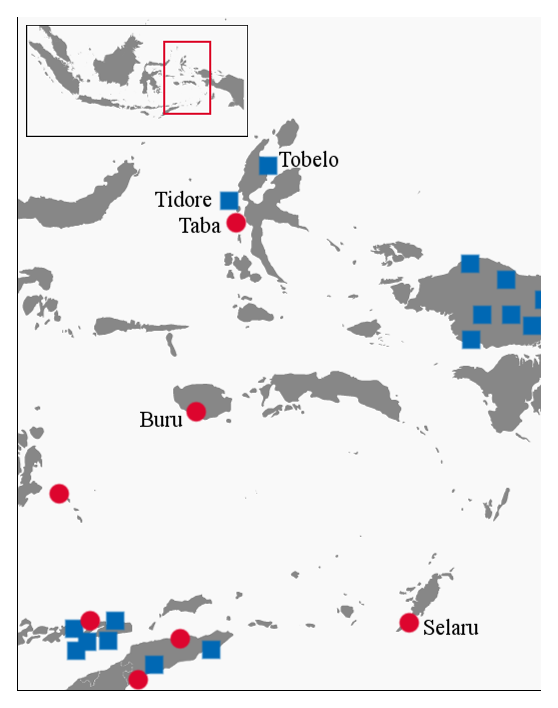
\includegraphics[width=0.55\textwidth]{../Maps/Map_Maluku2.eps}
\caption{Geographical distribution of languages from the Maluku subarea.}\label{map:Mal}
\end{center}
\end{figure}

Selaru is an Austronesian CMP languages with typical SV/AVO constituent order, prepositions and subject indexing by prefixes on the verb. Subject indexing is a regular process and each verb is marked by one of three inflectional classes, according to the stem onset. As in many of the TAP languages, animacy plays a role in Selaru. Inanimate subject referents are crossreferenced on the verb with a special prefix that is neutral with regard to number agreement. Consider the example below.

\ex \label{selaru1}
\begingl[glhangstyle=none]
\gla Toto, mbwa ti mal masire ma + kele ksyoyeta bakbakare // \rightcomment{{\small \textbf{Selaru} \textsc{mal}}}
\glb toto, mw-ba ti mw-al masy-Vre ma kele ky-soyeta bakbak-Vre //
\glc boy, \acs{2}\acs{sg}-go \acs{conj} \acs{2}\acs{sg}-get fish-\acs{pl} \acs{conj} then \acs{inan}-replace dry-\acs{pl} //
\glft `Boy, you go and get some fish in order to replace the dried ones.‘ \trailingcitation{{\small (Coward 2005: 66)}}// 
\endgl
\xe

While the animate subject is indexed on each of the first two verbs by the second person singular prefix \textit{mw-}, the fish from the second VP is reintroduced as the subject of the following clause by use of the inanimate prefix \textit{ky-}. 

Another peculiar feature of Selaru is that MVCs are infrequent and occur in rather unexpected types. One reason for this is that Selaru employs two semantically unspecific linkers, \textit{ti} and \textit{ma}, both of which appear to be grammaticalised from motion verbs\footnote{The origin of \textit{ma} seems clear from a vast range of surrounding Austronesian and Papuan languages many of which still show reflexes of a reconstructable motion verb *mai 'come' (Ross et al. 2008 give PAn *maRi, *mai 'come', PCEMP *mai 'come' and POc *mai, *ma 'come'/'DIR (towards speaker)'. The origin of \textit{ti} is less clear. In \ili{Waima'a}, there is a motion goal verb \textit{tii} meaning 'arrive' or 'until' in a temporal sense, and Tetun Fehan has \textit{ti'a} meaning 'already' both of which are reminiscent of Indonesian \textit{tiba} 'arrive' but I have not come across any proposed reconstruction. Selaru seems to use a verb stem \textit{-ait} for 'arrive' (Coward 2005: 175).}. These linkers appear in most contexts where in other languages of the EI area we would find unmarked verb sequences. Example (\ref{selaru1}) from above illustrates this nicely with the motion - action sequence \textit{mbwa ti mal} that in virtually all other languages would be expressed by a plain MVC, yet in Selaru one of the two markers overtly chains the two verbs together. Apart from the low functionality of MVCs, Selaru is a rather typical representative of an Eastern Indonesian language, showing for instance possessive classification with alienable and inalienable constructions (the former of which marks a further split into edible and non-edible possessums) and object preposing (functionally similar to passive alternations, although there is no real voice distinction in Selaru). 

Buru is in some ways similar to Selaru, including the overall scarcity of MVCs, although Grimes (1991) reports on a range of MVC types. In contrast to Selaru and the other languages included in the Maluku subsample, Buru has lost all inflecting devices on the verb (while retaining a rather elaborate set of derivational prefixes and suffixes). Buru is therefore from a verb-morphological perspective more similar to \ili{Waima'a} and Alorese than it is to Selaru.

The other three languages from the Maluku group are both spoken on Halmahera and surrounding islands. Taba (or East Makian) is another Austronesian language, genealogically belonging to the South Halmahera-West New Guinea branch and showing the by now familiar Austronesian word order pattern SV/AVO. Bowden (2001: 144f.) points out that while Taba meets most of the typological expectations connected to word order-correlations in VO languages, it does show some sign of deviation, most prominently from the preposed possessor order that Himmelmann (2005c) argued to be a general trait of Eastern Indonesian (Austronesian) languages (see section §\ref{sec:preposed}). Actor arguments are expressed by crossreferencing prefixes on the verb. Having a split-S system, this pertains in Taba to A and S$_A$ arguments. Undergoer S$_O$ arguments are not subject to verbal indexing though pronominal S$_O$ arguments are placed in postverbal position instead of expected SV. This split leads in some examples of MVCs to interesting constructions where the participant is marked twice, one time as the actor and one time as the undergoer. Consider the following example:

\ex \label{taba1}
\begingl
\gla nwosal máddodang i // \rightcomment{{\small \textbf{Taba} \textsc{mal}}}
\glb n=wosal máddodang i //
\glc \acs{3}\acs{sg}=stand be.straight \acs{3}\acs{sg} //
\glft `He's standing up straight' \trailingcitation{{\small (Bowden 2001: 300f.)}}// 
\endgl
\xe

The postposed pronoun \textit{i}, which is optional here, denotes by its specific distribution a S$_O$ argument. This argument must be understood as being coreferential with the S$_A$ argument indexed on the first verb. This construction is thus similar to reflexive and middle voice constructions (Bowden 2001: 301), and is mirrored in Taba by another peculiar construction. Verbs of excretion in Taba not only show an indexed actor argument but also a set of suffixes that are otherwise completely absent from that language. Compare example (\ref{taba2}).

\ex \label{taba2}
\begingl
\gla Buang nciwi // \rightcomment{{\small \textbf{Taba} \textsc{mal}}}
\glb Buang n=sio-i //
\glc Buang \acs{3}\acs{sg}=shit-\acs{3}\acs{sg} //
\glft `Buang shitted' \trailingcitation{{\small (Bowden 2001: 196)}}// 
\endgl
\xe

Just as in (\ref{taba1}), we see that a single participant receives actor and undergoer encoding at the same time. A similar, albeit distinct, construction is also found in Tobelo, one of the Papuan languages that form the closely related Northeast Halmaheran group. 

Tobelo retains many Papuan features, including conservative SV/AOV word order, postpositions, gender (male, female, non-human) and noun markers. Core-arguments are indexed on the verb by two sets of prefixes (called subjective and objective paradigm respectively, see Holton 2003: 38). The single argument of active intransitives as well as the A argument of transitives are indexed by the subjective paradigm occupying the initial prefix slot. The single argument of stative intransitives and the O argument of transitives, on the other hand, are marked in the second prefix slot by the objective paradigm. Example (\ref{tobelo1}) illustrates a minimal transitive construction in Tobelo (ellipsis being common for topical arguments).

\ex \label{tobelo1}
\begingl
\gla i-hi-goli // \rightcomment{{\small \textbf{Tobelo} \textsc{mal}}}
\glb 3-1-bite //
\glft `It/they bit me' \trailingcitation{{\small (Holton 2003: 39)}}// 
\endgl
\xe

Now, there is a further quirk in Tobelo's active-stative system in that the stative intransitives appear to be encoded just like transitive predicates. While the S$_O$ argument is indexed by the objective paradigm in the second slot, the first slot invariably shows neutral third person singular \textit{i-}, effecting some kind of pseudo-transitive construction. Compare the following example:

\ex \label{}
\begingl
\gla i-hi-pehaka // \rightcomment{{\small \textbf{Tobelo} \textsc{mal}}}
\glb 3-1-wet //
\glft `I am wet' \trailingcitation{{\small (Holton 2003: 38)}}// 
\endgl
\xe

While the Taba excretion construction can be formally differentiated from Tobelo stative instransitives by the fact that the former shows person and number agreement in both markers while the latter always has 3SG.NH for the `actor', the gist is that in both systems the referent appears to lack full control of the situation which is apparently what is captured by the undergoer marking here.

Tobelo has an array of further formatives appearing on the verb, such as applicative, distributive, intensifier morphology as well as a set of aspect suffixes denoting perfective, imperfective, repetitive, durative, and sequential events. These aspect suffixes are not obligatory, and do not form a viewpoint aspect system such as in the classical Russian case. They may occasionally also attach to host classes other than verbs (for instance to nouns and numerals). This makes Tobelo aspect suffixes category-independent (Holton 2003: 44), which casts doubt on the usefulness of theses suffixes as indicators of finiteness in verbs. 

Tidore, another Papuan language of Halmahera, is morphologically less elaborate than Tobelo. Tidore verbs may take a subject prefix\footnote{In van Staden's grammar on Tidore, this prefix is called `actor prefix'. It appears, however, that clear undergoer verbs such as 'fall' or `(be) drunk' also accept the prefix (see for instance example (\ref{Tidore1})). Two distinct person-marking paradigms that would convey differences in semantic roles, as we find in Tobelo, are missing in Tidore. In the examples from Tidore I left the \textsc{act} gloss in place though I do understand the prefix set as agreeing more generally to any argument in subject function.} inflecting for person, number (and partially for gender and animacy). Argument indexing, however, seems to be completely optional, without any apparent change as to wellformedness or sociolectal situation. Based on a small exploratory analysis of 80 turntaking units from one conversation, van Staden (2000: 79) reports that only about one third of all inflectible main verbs actually take an argument indexer. A verb that stays uninflected may thus be uninflected for two reasons: it may either be uninflected simply by pragmatic choice, or through grammatical restrictions. For instance, in the example pair (\ref{Tidore1}), the second verb \textit{tora} remains uninflected because of constructional constraints. The first verb, on the other hand, is free to accept a person marker or to remain bare.

\pex \label{Tidore1}
\a
\begingl
\gla ngofa ngge peka tora // \rightcomment{{\small \textbf{Tidore} \textsc{mal}}}
\glb child 3\acs{nhum}.there fall go.downwards //
\glft `the child fell down’ // 
\endgl
\a
\begingl
\gla ngofa ngge yo-peka tora // 
\glb child 3\acs{nhum}.there 3\acs{nhum}.\acs{act}-fall go.downwards //
\glft  \trailingcitation{{\small (van Staden 2000: 81)}}// 
\endgl
\xe

Table \ref{table:overviewmaluku} summarizes some of the core features associated with the verb systems of the Maluku subgroup.

\begin{table}[h]
\begin{center}
\begin{footnotesize}
\begin{tabular}{l r r r}
\hline\hline
language & constituent order & argument indexing & other verbal inflection \tabularnewline
\hline
Buru & SV, AVO & -- & -- \tabularnewline
Selaru & SV, AVO & S/A & -- \tabularnewline
Taba & SV, AVO & S$_A$/A & -- \tabularnewline
Tidore & SV, AVO & (S/A) & -- \tabularnewline
Tobelo & SV, AOV & S$_A$/A, S$_O$/O & aspect? \tabularnewline
\hline
\end{tabular}
\caption[Basic features of Maluku verb systems]{Overview of basic verbal features of the Maluku languages in the EI data set. Constituent order lists only the basic pattern, pragmatically induced alternative patterns are often also available. Brackets indicate optional use of argument indexers.}
\label{table:overviewmaluku}
\end{footnotesize}
\end{center}
\end{table}
\FloatBarrier

\subsection{Western Papua}\label{sec:westpapua2}

The last subarea is comprised of the westernmost part of mainland New Guinea: the Bird's Head peninsula down to Bintuni Bay, as well as the islands of Cenderawasih Bay to the east. The Bird's Head is a geographically diverse peninsula, ranging from the vast mangrove swamps in the Bintuni Bay area to the Tamrau and Arfak Mountains towering up in the north and east. The region is home to a couple of Papuan language families as well as to the West New Guina-subbranch of the Austronesian SHWNG phylum. As with the Nusa Tenggara group, I included 11 languages from this region in the dataset. 

\begin{figure}
\begin{center}
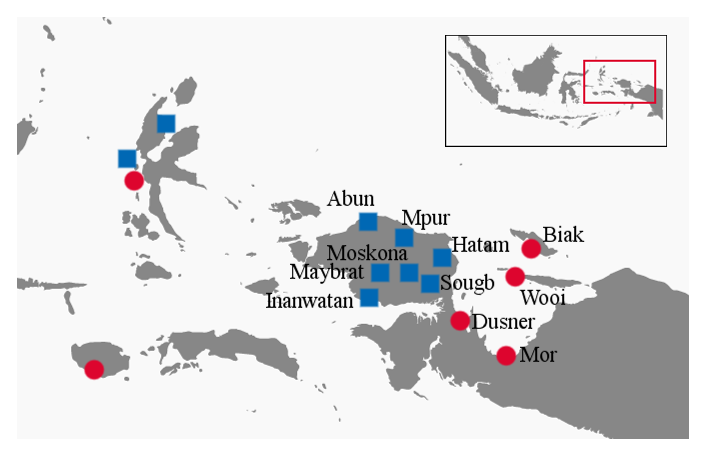
\includegraphics[width=0.7\textwidth]{../Maps/Map_Papua2.eps}
\caption{Distribution of languages from the Western Papua subarea.}\label{map:Pap}
\end{center}
\end{figure}

I will discuss these languages in three groups. The first group includes the Papuan family-level isolates Abun, Mpur and Maybrat, as well as the \acs{SBH} language Inanwatan. The languages of this group are all spoken in the north and west of the Bird's Head, Abun and Mpur along the northern coastline, Maybrat further inland on the central plateau, at the foothills of the Tamrau mountain range, and Inanwatan along the southwestern coast. The second group of languages is formed by members of the EBH family and the Hatam-Mansim family. They are all located in the eastern part of the Bird's Head. Third and last comes the group of Austronesian languages, including Biak, Dusner, Mor and Wooi which are all located in the Cenderawasih Bay area.

A few typological features apply to (almost) all these languages (which is why Reesink (2005) speaks of West Papuan languages in a geographical sense) and can be discussed together. Constituent order in WP  and the Austronesian languages is almost invariably SV/AVO with only Inanwatan showing Papuan AOV order (though direct objects may be placed postverbally, see Reesink 2005: 195, also de Vries 2004: 52f.). Almost all languages in the area have argument indexing prefixes on the verb (except Abun; Dol 2007: 5). Gender is a persistent feature only in the first group (except for Abun), and lacking in the \acs{EBH} family, in Hatam and in the Austronesian languages (Reesink 2005: 205). A further syntactic hallmark is the placement of the negator which is clause-final, or at least post-predicate (Reesink 2005: 199), tallying well with Himmelmann's  preposed possessor type in Austronesian languages of the area. The high degree of mutual influence between Papuan and Austronesian languages is also witnessed by strikingly similar phonemic shapes of the negators, many of them corresponding to a form \#\textit{va/\textipa{\textbeta}a} or \#\textit{te} (see Reesink 2005: 199 for discussion).

The three family-isolate languages of the first group, Abun, Mpur and Maybrat, do not have any established genealogical context and hence are sufficiently different from each other in terms of lexical and grammatical properties\footnote{Maybrat has in fact been linked to the \acs{WBH} family (of which no language could be included in the present data set), with traces of cognate structures in pronouns, gender distinction, and verbal prepositions (Reesink 2005: 187).}. Inanwatan, on the other hand, as a member of the SBH family, provides some evidence for a distant relationship to the TNG language family. 

Of all WP languages, Abun ``seems to have undergone the highest degree of morphological erosion, even to the extent that verbal affixation is totally absent" (Reesink 2005: 205). Instead of verbal morphology, many grammatical features in Abun are encoded by particles. As there is no argument indexing on the verb nor any case marking, Abun grammatical relations are entirely defined by position, i.e., the subject is always that NP that stands before the predicate (Berry and Berry 1999: 48). Objects may be fronted if topicalised, and they are also frequently subject of ellipsis (1999: 51). While SVCs do not constitute a distinct topic in Berry and Berry's grammar, they do note in passing that SVCs are not uncommon in Abun and that there is some variation between speakers as to the placement of pronouns ``to separate verbs" (1999: 51f.). Examples (\ref{abun1a}) and (\ref{abun1b}) serve to illustrate the basic linguistic structure of Abun clauses, as well as interverbal pronoun placement in SVCs. Note that both constructions involve a motion-to-action sequence, yet the coding differs in both cases according to the presence or absence of subject marking of V$_2$. While the first case looks like two juxtaposed clauses and thus arguably corresponds to the Kambera control construction using \textit{pa-}, or to the Selaru linker construction, the second case is the expected unmarked construction that is typical for most of the other languages of EI.

\pex 
\a \label{abun1a}
\begingl
\gla ji mu ji git su-git mo nu // \rightcomment{{\small \textbf{Abun} \textsc{pap}}}
\glb \acs{1}\acs{sg} go \acs{1}\acs{sg} eat \acs{nmlz}-eat \acs{loc} house //
\glft 'I went and ate at home' // 
\endgl
\a \label{abun1b}
\begingl
\gla ye-suk-mise ma nai gwat an mu ket // 
\glb \acs{pers}-\acs{nmlz}-evil come capture carry \acs{3}\acs{sg} go west //
\glft `The police came and caught him and took him westward' \trailingcitation{{\small (Berry and Berry 1999: 52)}}// 
\endgl
\xe

Mpur, Maybrat and Inanwatan, on the other hand, function quite differently and index S/A arguments or S/A and O arguments (Inanwatan) on the verb. Mpur has S/A-indexing prefixes but indexing is only obligatory with human subjects. The 3SG indexer shows a gender split into a masculine and a feminine form. The Mpur pattern is paralleled in Maybrat with the difference that the non-masculine gender is the unmarked gender associated with most nouns (i.e. those without male sexus), and the indexing system appears to be obligatory with all kinds of referents. Bisyllabic verb stems in Maybrat that have a C-initial second syllable do not, however, take overt person prefixes but may be analysed as covertly inflecting for person (see Dol 2007: 52f. for discussion).

Inanwatan is morphologically more complex and has a linguistic profile that is similar to that of the Marind languages from the south central coast of New Guinea suggesting an old genealogical relationship (de Vries  2004: 16). De Vries notes that the Marind languages have four characteristic features that are also present in Inanwatan: (i) subject prefix followed by object prefix on the verb in a basic AOV clause; (ii) suppletive verb stems indicating plurality of the subject (and sometimes of the object); (iii) gender systems with agreement phenomena and with front vowels indicating masculine and back vowels indicating feminine gender; and (iv) coordination of fully inflected verbs instead of clause chaining with medial verbs, and no or marginal presence of serial verbs. The following examples illustrate properties (i) and (iii), respectively.

\pex 
\a \label{inan1o}
\begingl
\gla iwáa-go suqére né-i-we-re // \rightcomment{{\small \textbf{Inanwatan} \textsc{pap}}}
\glb yesterday-\acs{circ} sago \acs{1}\acs{sg}.\acs{subj}-\acs{2}\acs{pl}.\acs{obj}-give-\acs{pst} //
\glft `Yesterday I gave you sago' // 
\endgl
\a \label{inan2o}
\begingl[glhangstyle=none]
\gla nó-opo-be-re + né-ri-be-re né-re-be // 
\glb \acs{1}\acs{sg}.\acs{subj}-take.a.bath-\acs{pres}-and \acs{1}\acs{sg}.\acs{subj}-eat-\acs{pres}-and \acs{1}\acs{sg}.\acs{subj}-sleep-\acs{pres} //
\glft `I took a bath, ate and slept' \trailingcitation{{\small (de Vries 2004: 15)}}// 
\endgl
\xe

Example (\ref{inan1o}) shows the order of indexers on a ditransitive verb with A and G being indexed while the T argument is only expressed via an NP. Generally, O and G indexing only happens when the object is either the speaker or the addressee, otherwise only S/A is marked on the verb (de Vries 2004: 35). Inanwatan has another two categories that cause inflection on the verb. First, there are three tenses, past, present and future tense, each marked by a tense suffix. And second, there is the habitual-durative suffix \textit{-rita} (the only aspectual distinction marked that way) replacing the tense suffixes in events that occur habitually, repeatedly or prolonged (de Vries 2004: 38).

The second example in (\ref{inan2o}) is an instance of Inanwatan clause coordination, a feature that is only marginally (if at all) present in other WP and Austronesian languages of the area. Event sequences of a similar sort may be found in other languages as well, though without overt coordination morphology. There are, however, other multi-verb sequences in Inanwatan that do not receive such coordination marking.

The three languages of the second group, Hatam, Sougb and Moskona, are structurally rather similar. They are all SV/AVO and they have subject prefixes on the verb. Otherwise their verbal morphology is quite simple. Gender as a nominal category is absent from Moskona, but there is a phonological distinction into alienable and inalienable nouns in that members of the former group begin with \textit{m-}. Subject arguments are crossreferenced on the verb and may be omitted if topical (Gravelle 2010: 269), objects follow their verb and can be moved to a pre-posed topic position as is common throughout the area. Moskona also marks irrealis on the verb by using the prefix \textit{me-/m-}. The irrealis marker comes after the subject prefix and before a potential causative prefix. In negative polarity clauses, the verb always takes \textit{me-} (Gravelle 2010: 110). 

Related Sougb also has the Moskona features except for some minor differences: alienable nouns do not show a fossilised \textit{m-} prefix but instead inalienable nouns appear to begin with a vowel (Reesink 2002b: 218). Verbs in Sougb are also phonologically restricted and begin with a [-\textsc{high}] vowel, either /e/, /o/ or /a/. Sougb verbs may take subject indexing prefixes, the irrealis morpheme \textit{em-} and the instrument marker \textit{a-}, and the combination of these prefixes differs in the three verb classes with regard to vowel realisation in the stem and the prefixes (Reesink 2002b). The instrument marker is a phenomenon that occurs in a range of languages in the area (also Austronesian ones) and has repercussions for SVC analysis. I repeat two examples of the use of the instrumental prefix from Reesink (2002b) below:

\pex 
\a
\begingl
\gla dan d-eic kepta d-a-(e)hi sogo // \rightcomment{{\small \textbf{Sougb} \textsc{pap}}}
\glb I \acs{1}\acs{sg}-take machete \acs{1}\acs{sg}-\acs{ins}-fell tree //
\glft `I cut the tree with a machete' // 
\endgl
\a \label{sougb1}
\begingl
\gla dan d-et roti d-a-(e)k kopi // 
\glb I \acs{1}\acs{sg}-eat bread \acs{1}\acs{sg}-\acs{ins}-drink coffee //
\glft `I eat bread and drink coffee' \trailingcitation{{\small (Reesink 2002b: 205)}}// 
\endgl
\xe

In the first example, a sequence of two verbs, \textit{eic} `take' and \textit{ehi} `fell' is connected by the use of the instrument prefix reanalysing the T argument of the first verb as the instrument of the second. Take-action sequences are quite common throughout EI but the instrument prefix here adds specific morphology to the construction disambiguating its status as a coherent unit as it seems. This is in contrast to other languages, especially in the \textsc{nus} region, where the verbs are merely juxtaposed without overt argument-flagging. The second example in (\ref{sougb1}) is different as the use of the instrument marker here seems to follow from the fact that ``a previous predicate has introduced an instrument or an accompaniement" (Reesink 2002: 205). One might wonder, however, whether a reading like ``I eat bread and drink it by dipping it into the coffee" would not be preferred here.

Neighbouring Hatam also has an instrument prefix that appears on verbs in verb sequences. In fact, there are two homophonous morphemes \textit{bi-} that seem to express quite related concepts though they clearly occupy different preverbal slots. While the instrumental \textit{bi-} appears after the person prefix and before the root, purposive \textit{bi-} comes first in sequence right before the person prefix. The following example illustrates both items in their morphological context.

\ex \label{}
\begingl[glhangstyle=none]
\gla yoni i-ba micim i-bi-dat + dani bigom bi-di-mai // \rightcomment{{\small \textbf{Hatam} \textsc{pap}}}
\glb they \acs{3}\acs{pl}-take spear \acs{3}\acs{pl}-\acs{ins}-pierce I almost \acs{purp}-\acs{1}\acs{sg}-die //
\glft `They almost killed me with their spear(s)' \trailingcitation{{\small (Reesink 1999: 103)}}// 
\endgl
\xe

The first instance of \textit{bi-} functions much the way Sougb \textit{a-} does: the O argument of a previous verb is flagged as instrument of the \textit{bi-}marked verb. Note that the subject of both verbs remains co-referential. In the second case there is no direct reanalysis of a previous argument. Rather what seems to be referred to with purposive \textit{bi-} is the whole previous proposition becoming the reason or source for the \textit{bi-}marked action to take place. Another feature of purposive \textit{bi-} is that a change in subjects from V$_1$ to V$_2$ is possible. A further difference between the two markers is that only with instrumental \textit{bi-} which takes up a previous argument the subject prefix marker on the verb may be dropped.

The last group to be discussed here is the Austronesian languages of Western Papua. Dusner and Biak are closely related. Both languages have reduced initial syllables in some roots leading to onset consonant clusters that are otherwise rare in Austronesia (for instance Biak \textit{mnu} 'village', cf. Wooi \textit{manu} 'house'). Wooi and Mor are phonologically simpler and have Austronesian CV(N) syllable structure. All language make use of person marking on the verb, indexing subjects with prefixes and infixes. Infixes occur in \textsc{2sg} and \textsc{3sg} in Wooi, Dusner and Biak (with consonant-inital verbs, otherwise as prefix) but not in Mor which has only prefixes (zero-marked for \textsc{3sg} on consonant-initial stems). Dusner and Biak have two \textsc{3pl} subject indexers. In Dusner, the split is between human and non-human, while in Biak animate subjects are distinguished from inanimates.

All languages are straightforward SV/AVO and frequently prepose objects. In Wooi, preposed objects need to be crossreferenced by bound resumptive object forms distinguishing between indiviuated object referents and non-individuated (plural) objects. In the following example, the hero Ayraroy (placed in preposed topic position) is killed by his enemies (and is resumptively referred to by the clitic \textit{=i}).

\ex \label{}
\begingl
\gla Ayraroy hemuni // \rightcomment{{\small \textbf{Wooi} \textsc{pap}}}
\glb A. he-mung=i //
\glc A. \acs{3}\acs{pl}-kill-\acs{3}\acs{sg}.\acs{obj} //
\glft `They killed Ayraroy' \trailingcitation{{\small (ethnic\_war\_1 081)}}// 
\endgl
\xe

Further features of the Austronesian group include clause-final negators, complex determiner and directional systems, instrument prefixes (much like in the EBH languages and in Hatam), as well as prepositions and clause linkers/topic markers developed from verbs. Serialisation seems quite pervasive although there is some variation between Wooi, showing many types of serial verbs, and for instance Biak, where serial verbs are mostly limited to cause-result sequences. Table \ref{table:overviewpapua} lists the crucial syntactic features.

\begin{table}[h]
\begin{center}
\begin{footnotesize}
\begin{tabular}{l r r r}
\hline\hline
language & constituent order & person marking & other verbal inflection \tabularnewline
\hline
Abun & SV,AVO & -- & -- \tabularnewline
Maybrat & SV, AVO & S/A & -- \tabularnewline
Mpur & SV, AVO & S/A & -- \tabularnewline
Inanwatan & SV, AOV & S/A, (O) & tense, aspect \tabularnewline
\hline
Moskona & SV, AVO & S/A & irrealis \tabularnewline
Sougb & SV, AVO & S/A & irrealis, instrument \tabularnewline
Hatam & SV, AVO & S/A & instrument \tabularnewline
\hline
Biak & SV, AVO & S/A & instrument \tabularnewline
Dusner & SV, AVO & S/A & instrument \tabularnewline
Wooi & SV, AVO & S/A & instrument \tabularnewline
Mor & SV, AVO & S/A & -- \tabularnewline
\hline
\end{tabular}
\caption[Basic verbal features of the Western Papuan languages]{Overview of basic verbal features of the Western Papuan languages in the data set. Constituent order lists only the basic pattern, pragmatically induced alternative patterns are often also possible.}
\label{table:overviewpapua}
\end{footnotesize}
\end{center}
\end{table}
\FloatBarrier

\section{Summary}

Summarizing the findings from this chapter, we have seen that most of the languages of EI, although genealogically and typologically quite varied, share some basic features, such as argument indexing on the verb and clause-final negation. The Papuan languages appear to fall into at least two areal clusters (leaving aside the North Halmahera languages): the TAP languages are verb-final languages with reduced and irregular undergoer argument indexing on part of their verbs. The West Papuan languages in the Bird's Head area, on the other hand, have converged on a couple of Austronesian features, such as adopting AVO word order and the inclusive/exclusive opposition. The Austronesian languages are more heterogeneous if we take into account the Sulawesi languages, the western outlier Kambera of \textsc{nus} or the highly isolating languages on Timor, such as \ili{Waima'a}. If we abstract away a little further we may imagine the languages of EI along a west-to-east gradient as tending to lose verbal morphology up to Timor and gaining or preserving verbal morphology yet further to the east in the Northern Moluccas and Western Papua. While person marking appears to be quite constant throughout, TAM marking is prevalent only in the far west and the far east of the area, leaving Nusa Tenggara practically devoid of these verbal categories.

This review has focused on verb morphology for two reasons: first, languages differ as to which categories are marked on the verbs. Second, languages strongly differ in the extent to which verb morphology is used. The challenge here is not only the lack of overt morphology in isolating languages, but also that a set of languages does not have \emph{reliable} verb morphology in the sense that in annotating verbal inflection in MVCs one is not able to determine whether a given verb is inflected, would potentially be inflected (if it had other lexical or phonological properties), or is in fact uninflected. I will come back to the issue of verb inflectability in chapter \ref{ch:gram}, where I will have another look at `unreliable inflection'.

In the next chapter, I will turn to the literature on verb serialisation, and explore in more detail the ways in which these constructions may be conceived of as coherent units. The chapter will then go on to explore the term MVC that is, I will argue, more suitable  for an analysis of the EI dataset than `verb serialisation', or my introductory term `underspecified verb sequences'.